%%!TEX encoding = UTF-8 Unicode

% Several lines in file have comments suggesting common packages for the
% typical thesis in informatics or electronics developed at UA
% uncomment/comment the lines as required for your work
% Before each optional line you will have a small comment

% According to UA rules, font size should range from 10 to 12pt.
\documentclass[11pt,a4paper,openright,twoside,onecolumn]{memoir}

\listfiles
\fixpdflayout

\usepackage[utf8]{inputenc}

% Select Computer Modern Typewritter (For bold ttfamily in listings)
\usepackage{lmodern}
% OR... Bera Mono
%\usepackage[scaled]{beramono} % TTT Font
%\usepackage{anyfontsize} % As the name says...

\usepackage[T1]{fontenc}

% Enable for for Overleaf support
\usepackage{ifthen}
\def\useoverleaf{0}  % change to non-zero (for instance, 1) to enable it

\makeatletter
\newcommand{\makecoverfile}[0]{%
  \immediate\write18{latexmk -pdf cover.tex}%
}
\makeatother

% For PDF merging
\usepackage{pdfpages}

% Set DPI to 300
\pdfpxdimen=\dimexpr 1in/300\relax

% Allow the use of a larger number of packages
\usepackage{morewrites} 

% For English and Portuguese languages
% Portuguese will be the default.
% Uncomment \setlanguage below to change it
\usepackage[english,portuguese]{babel}

% Uncomment to use a custom date format
%\usepackage{datetime}
%\newdateformat{thesisdate}{\monthname[\THEMONTH] \THEYEAR} % Month Year

% Make pdf look better
\usepackage{microtype} 

% Uncomment to enable floats on facing pages
%\usepackage{dpfloat}

% Side by side figures
% Eg. Fig 1a, Fig 1b
\usepackage[hang,small,bf]{caption}
%\let\tion\undefined
%\let\subfloat\undefined
\usepackage{subcaption}

%\RequirePackage{textcase}

% Dropped Caps
%\usepackage{lettrine}

% Configure Hyperlink color
% As a matter or style, you may use this to enable/disable color boxes on links
%\usepackage[breaklinks=true,colorlinks=false,linkcolor=blue]{hyperref}
% Or use the default values provided by the hyperref package
\usepackage{hyperref}

% Redefine section names according to your preference
%\def\sectionautorefname{Section}
%\def\chapterautorefname{Chapter}
%\def\figureautorefname{Figure}
%\def\listingautorefname{Listing}
%\def\tableautorefname{Table}

% Redefine code boxes
\ifthenelse{\equal{\useoverleaf}{0}}
{\usepackage[outputdir=build]{minted}}
{\usepackage{minted}}%

\addto\captionsportuguese{%
  \renewcommand\listingscaption{Code}
}
\fvset{fontsize=\footnotesize} % Make Code blocks smaller than text
\usepackage{csquotes}

% Add support for PDF Comments
\usepackage{comment}
\ifthenelse{\equal{\useoverleaf}{0}}
{\usepackage{pdfcomment}}{}
\usepackage{bookmark} % New Bookmarks

% For Multiple columns in Glossary
\usepackage{multicol}

% Add support for Math symbols
\usepackage{amsmath}
\usepackage{amssymb}

% Add support for graphics
\usepackage{graphicx}

% Add support for Colors
\usepackage{xcolor}

% Add support for the Euro symbol
\usepackage{eurosym}

% Add support for missingfigure and todo
\usepackage{todonotes}

% Setup bibliography with Biber using IEEE style for proper UTF-8 support
\usepackage[backend=biber, style=ieee, sorting=none, natbib=true, mincitenames=1, maxcitenames=2]{biblatex}
\bibliography{bib/references.bib, bib/rfc.bib}

% Use acronyms
\usepackage[printonlyused]{acronym} % For acronyms

% Indenting the first paragraph after section start
\usepackage{indentfirst}

% For fixing listoflistings with memoir
\usepackage{xparse}

% Uncomment the next lines to enable chart support through pgf and tikz
% This may require you to install further packages in your Tex system
%\usepackage[version=0.96]{pgf}
%\usepackage{tikz}

% UML support
%\usepackage{pgf-umlsd}

% Trees, Arrows, Mindmaps and other popular objects
%\usetikzlibrary{arrows,shadows,trees,shapes,decorations,automata,backgrounds,petri,mindmap} % for pgf-umlsd

% Package to master SI units
\usepackage[detect-weight=true, binary-units=true]{siunitx}
% For Electric Circuits
%\sisetup{load-configurations = binary}

% Set Voltage direction accordingly
% Option : oldvoltagedirection,nooldvoltagedirection,RPvoltages,EFvoltages
% More information at: https://mirrors.ibiblio.org/CTAN/graphics/pgf/contrib/circuitikz/doc/circuitikzmanual.pdf
% By default this template is using the Old Voltage Direction
%\usepackage[oldvoltagedirection,american,cuteinductors,smartlabels]{circuitikz}
%\usetikzlibrary{calc}
%\ctikzset{bipoles/thickness=1}
%\ctikzset{bipoles/length=0.8cm}
%\ctikzset{bipoles/diode/height=.375}
%\ctikzset{bipoles/diode/width=.3}
%\ctikzset{tripoles/thyristor/height=.8}
%\ctikzset{tripoles/thyristor/width=1}
%\ctikzset{bipoles/vsourceam/height/.initial=.7}
%\ctikzset{bipoles/vsourceam/width/.initial=.7}
%\tikzstyle{every node}=[font=\small]
%\tikzstyle{every path}=[line width=0.8pt,line cap=round,line join=round]

% For inline TT text (e.g. code snippets)
\usepackage{verbatim}

% Frames around figures and allow force placement
\usepackage{float}

% Configure Float style
%\floatstyle{boxed}
%\restylefloat{table}
%\restylefloat{figure}
%\restylefloat{lstlisting}

% For test purposes you may use the lipsum package to create dummy text
\usepackage{lipsum} % REMOVE

%Keep floats inside section!
\usepackage[section]{placeins}
\let \oldsubsubsection \subsubsection
\renewcommand{\subsubsection}[2][]{
  \FloatBarrier
  \oldsubsubsection#1{#2}
}
\let \oldsubsection \subsection
\renewcommand{\subsection}[2][]{
  \FloatBarrier
  \oldsubsection#1{#2}
}
\let \oldsection \section
\renewcommand{\section}[2][]{
  \FloatBarrier
  \oldsection#1{#2}
}
\let \oldchapter \chapter
\renewcommand{\chapter}[2][]{
  \FloatBarrier
  \oldchapter#1{#2}
}

\usepackage{multirow}

% For creating a list of abbreviations.
\usepackage[%
nogroupskip=false,%
nonumberlist=true,%
nopostdot=true,%
% style=alttree,%
style=listdotted,%
% style=long,%
% style=super,%
shortcuts=abbreviations,%
% The "uathesis" style file is already adding the glossary into the
% table of contents.
toc=false,%
]{glossaries-extra}

% Include defined abbreviations


\newabbreviation
    {ir}
    {IR}
    {Information Retrieval}
\newcommand{\ir}{\gls{ir}}

\newabbreviation
    {tf}
    {TF}
    {Term Frequency}
\newcommand{\tf}{\gls{tf}}

\newabbreviation
    {idf}
    {IDF}
    {Inverse Document Frenquency}
\newcommand{\idf}{\gls{idf}}

\newabbreviation
    {tf-idf}
    {TF-IDF}
    {Term Frequency - Inverse Document Frenquency}
\newcommand{\tfidf}{\gls{tfidf}}

\newabbreviation
    {dl}
    {DL}
    {Document Length}
\newcommand{\dl}{\gls{dl}}


\newabbreviation
    {bm25}
    {BM25}
    {Best Matching 25}
\newcommand{\bm}{\gls{bm}}

\newabbreviation
    {qa}
    {QA}
    {Question Answering}
\newcommand{\qa}{\gls{qa}}

\newabbreviation
    {ai}
    {AI}
    {Artificial Intelligence}
\newcommand{\ai}{\gls{ai}}

\newabbreviation
    {nlp}
    {NLP}
    {Natural Language Processing}
\newcommand{\nlp}{\gls{nlp}}

\newabbreviation
    {nlu}
    {NLU}
    {Natural Language Understanding}
\newcommand{\nlu}{\gls{nlu}}

\newabbreviation
    {nlg}
    {NLG}
    {Natural Language Generation}
\newcommand{\nlg}{\gls{nlg}}

\newabbreviation
    {lm}
    {LM}
    {Language Models}
\newcommand{\lm}{\gls{lm}}

\newabbreviation
    {llm}
    {LLM}
    {Large Language Models}
\newcommand{\llm}{\gls{llm}}

\newabbreviation
    {slm}
    {SLM}
    {Statistical Language Models}
\newcommand{\slm}{\gls{slm}}

\newabbreviation
    {nlm}
    {NLM}
    {Neural Language Models}
\newcommand{\nlm}{\gls{nlm}}

\newabbreviation
    {plm}
    {PLM}
    {Pre-trained Language Models}
\newcommand{\plm}{\gls{plm}}

\newabbreviation
    {bert}
    {BERT}
    {Bidirectional Encoder Representations from Transformers}
\newcommand{\bert}{\gls{bert}}

\newabbreviation
    {gpt}
    {GPT}
    {Generative Pre-trained Transformer}
\newcommand{\gpt}{\gls{gpt}}

\newabbreviation
    {ml}
    {ML}
    {Machine Learning}
\newcommand{\mlearning}{\gls{mlearning}}

% \renewcommand{\glossaryname}{Glossary}


% Use the built-in division styling
\headstyles{memman}

% Include subsections in the TOC
\settocdepth{subsection}

% Numbering down to subsections as well
\setsecnumdepth{subsection}

% extra index for first lines
\makeindex[lines]

% Margins for University of Aveiro Thesis
\setlrmarginsandblock{3cm}{2.5cm}{*}
\setulmarginsandblock{3cm}{3cm}{*}
\checkandfixthelayout

% Or select your custom spacing to make any ajustment
%\addtolength{\parskip}{0.5\baselineskip}
\linespread{1.5}

\newcommand\mainmatterWithoutReset
{\edef\temppagenumber{\arabic{page}}%
  \mainmatter
  \setcounter{page}{\temppagenumber}%
}


%%%%%%%%%%%%%%%%%%%%%%%%%%%%%%%%%%%%%%%%%%%%%%%%%%
% Document begins here
%%%%%%%%%%%%%%%%%%%%%%%%%%%%%%%%%%%%%%%%%%%%%%%%%%

\begin{document}

% Fix the numbering scheme by having a ghost style for page numbering
\pagenumbering{Alph}

\ifthenelse{\equal{\useoverleaf}{0}}{}{\makecoverfile{}}%
%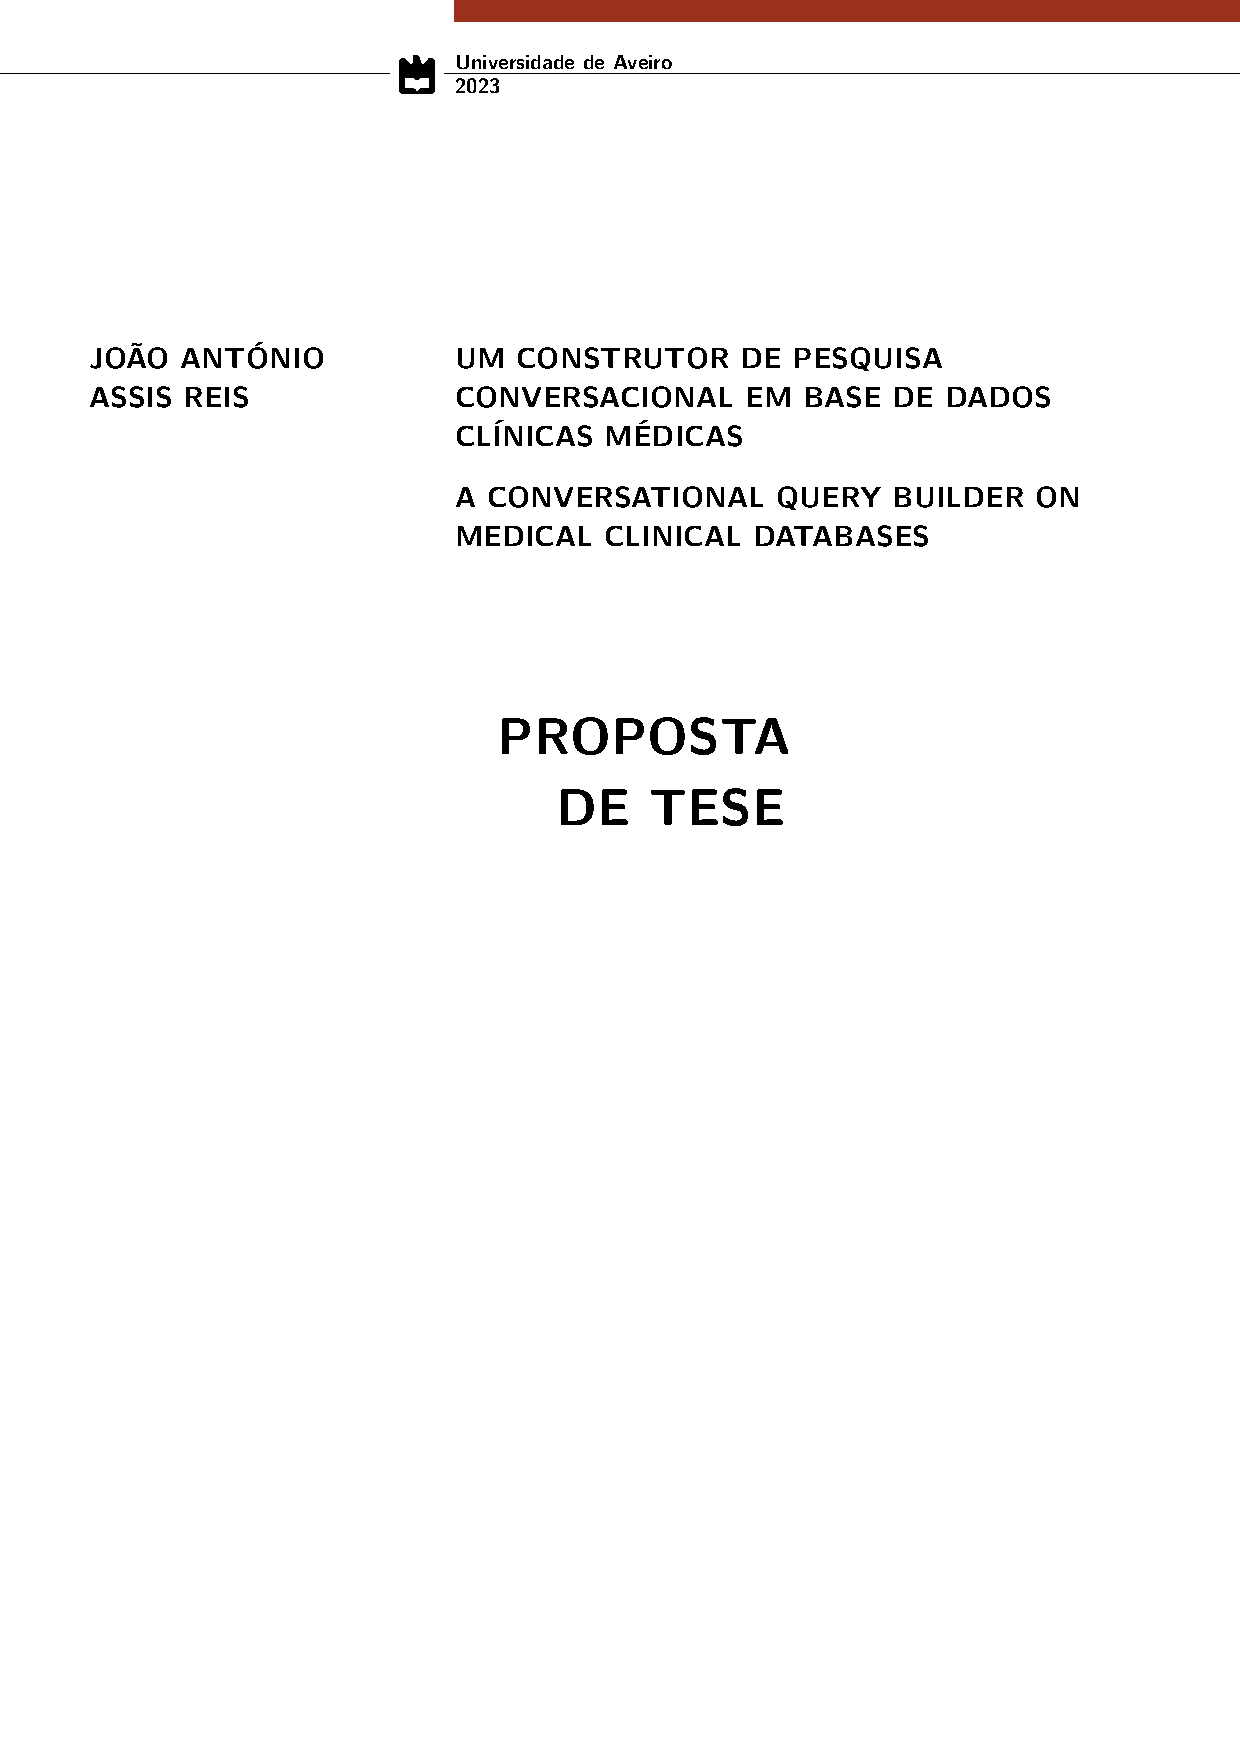
\includepdf[pages=-]{cover.pdf}

% Uncomment to enable English
\selectlanguage{english}


% Front matter

%Custom Chapter style named `thesis`
\makechapterstyle{thesis}{% Based on ell
  \chapterstyle{default}
  \renewcommand*{\chapnumfont}{\normalfont\sffamily}
  \renewcommand*{\chaptitlefont}{\normalfont\Huge\sffamily}
  \settowidth{\chapindent}{\chapnumfont 111}
  \renewcommand*{\chapterheadstart}{\begingroup
    \vspace*{\beforechapskip}%
    \begin{adjustwidth}{}{-\chapindent}%
    \hrulefill
    \smash{\rule{0.4pt}{15mm}}
    \end{adjustwidth}\endgroup}
  \renewcommand*{\printchaptername}{}
  \renewcommand*{\chapternamenum}{}
  \renewcommand*{\printchapternum}{%
    \begin{adjustwidth}{}{-\chapindent}
    \hfill
    \raisebox{10mm}[0pt][0pt]{\fontsize{30}{25}\selectfont\chapnumfont \thechapter}%
                              \hspace*{1em}
    \end{adjustwidth}\vspace*{-3.0\onelineskip}}
  \renewcommand*{\printchaptertitle}[1]{%
    \vskip\onelineskip
    \raggedleft {\chaptitlefont ##1}\par\nobreak\vskip 4\onelineskip}}


% Select chapter style from existing or select custom
%\chapterstyle{thesis} % Others: dowding, demo2, dash, chappell, brotherton, bianchi, ger, madsen, tatcher, veelo,indexes)
% thesis can also be used as defined previously
% Check the memoir documentation for the available themes
% Default is veelo
\chapterstyle{veelo}
\makeoddfoot{plain}{}{\thepage}{} % Added by André Zúquete to fix a page numbering issue on the veelo chapter style


% If you feel adventurous you can also define all aspects of your theme
% Use either this input or the chapterstyle before
% % Rules
\newcommand{\thinRule}{\rule{\textwidth}{0.25pt}}

% Customize heading appearances
% Define styles
\newcommand{\partSize}{\Huge}
\newcommand{\partStyle}{\lsstyle\scshape}
\newcommand{\chapterSize}{\Huge}
\newcommand{\chapterStyle}{\lsstyle\scshape}
\newcommand{\chapterAfter}{}
\newcommand{\sectionSize}{\Large}
\newcommand{\sectionStyle}{\scshape\MakeTextLowercase}
\newcommand{\subsectionSize}{\large}
\newcommand{\subsectionStyle}{\scshape\MakeTextLowercase}
\newcommand{\subsubsectionSize}{\large}
\newcommand{\subsubsectionStyle}{\scshape\MakeTextLowercase}
\newlength{\partNumSizePt}
\setlength{\partNumSizePt}{60pt}
\newlength{\chapterNumSizePt}
\setlength{\chapterNumSizePt}{60pt}
\newcommand{\partNumSize}{%
  \fontsize{\partNumSizePt}{1.2\partNumSizePt}\selectfont%
}
\newcommand{\partNumStyle}{\partChapterNumColor}
\newcommand{\chapterNumSize}{%
  \fontsize{\chapterNumSizePt}{1.2\chapterNumSizePt}\selectfont%
}
\newcommand{\chapterNumStyle}{\partChapterNumColor}

% Customize parts
\renewcommand{\partnamefont}{\partSize\partStyle}
\renewcommand{\partnumfont}{\partNumSize\partNumStyle}
\renewcommand{\printpartname}{}
\renewcommand{\printparttitle}[1]{%
  \normalfont\normalcolor\partnamefont #1
}

% Customize chapters
\makeatletter
\setlength{\beforechapskip}{30pt}
\renewcommand*{\chapterheadstart}{\vspace*{\beforechapskip}}
\setlength{\afterchapskip}{3ex}
\setlength{\midchapskip}{3ex}
\renewcommand*{\chapnamefont}{%
  \Large\flushright\chapterStyle\partChapterNumColor%
}
\renewcommand*{\chapnumfont}{\chapterNumSize\chapterNumStyle}
\renewcommand*{\chaptitlefont}{%
  \normalfont\flushleft\normalcolor\chapterSize\chapterStyle%
}
\renewcommand*{\printchaptername}{%
  \chapnamefont\MakeTextLowercase{\@chapapp}%
}
\renewcommand*{\chapternamenum}{\quad}
\renewcommand*{\printchapternum}{%
%  \chapnumfont\textls[-75]{\classicstylenums{\thechapter}}%
 \chapnumfont\textls[-75]{\thechapter}%

}
\renewcommand*{\printchaptertitle}[1]{%
  \chaptitlefont #1
  \chapterAfter
}
\makeatother
% Customize sections and subsections
\setsecnumformat{\csname my#1\endcsname\quad}
\setsecheadstyle{\sectionSize\sectionStyle}
\newcommand{\mysection}{{\thesection}}
\setlength{\beforesecskip}{3em}


\setsubsecheadstyle{\subsectionSize\subsectionStyle}
\newcommand{\mysubsection}{{\normalfont\subsectionSize\thesubsection}}
\setlength{\beforesubsecskip}{3em}

\setsubsubsecheadstyle{\subsubsectionSize\subsubsectionStyle}
\newcommand{\mysubsubsection}{{\normalfont\subsubsectionSize\thesubsubsection}}
\setlength{\beforesubsubsecskip}{2em}

% Customize "Table of ..." appearance
% Customize headings
\newcommand{\renewPrintXTitle}[1]{%
  \renewcommand{#1}[1]{%
    \printchaptertitle{##1}%
  }%
}
\renewPrintXTitle{\printtoctitle}
\renewPrintXTitle{\printlottitle}
\renewPrintXTitle{\printloftitle}

% Customize ToC headings
\renewcommand{\cftpartfont}{\partChapterNumColor\partStyle}
\renewcommand{\cftchapterfont}{\chapterStyle}
\renewcommand{\cftsectionfont}{}
\renewcommand{\cftsubsectionfont}{}
\renewcommand{\cftfigurefont}{}
\renewcommand{\cfttablefont}{}
\newcommand{\cftlstlistingfont}{}

% Increase number width
\newlength{\cftNumWidthIncrease}
\setlength{\cftNumWidthIncrease}{0.25em}
\addtolength{\cftpartnumwidth}{\cftNumWidthIncrease}
\addtolength{\cftchapternumwidth}{\cftNumWidthIncrease}
\addtolength{\cftsectionindent}{\cftNumWidthIncrease}
\addtolength{\cftsubsectionindent}{\cftNumWidthIncrease}
% No leader dots
%\renewcommand*{\cftpartdotsep}{\cftnodots}
%\renewcommand*{\cftchapterdotsep}{\cftnodots}
%\renewcommand*{\cftsectiondotsep}{\cftnodots}
%\renewcommand*{\cftsubsectiondotsep}{\cftnodots}
%\renewcommand*{\cftfiguredotsep}{\cftnodots}
%\renewcommand*{\cfttabledotsep}{\cftnodots}
%\newcommand*{\cftlstlistingdotsep}{\cftnodots}
% Set page numbers immediately after entry text
\newcommand{\tocEntryPageSep}{\hspace{1em}}
\renewcommand{\cftpartleader}{\cftdotfill{\cftdotsep}}
%\renewcommand{\cftpartafterpnum}{\cftparfillskip}
%\renewcommand{\cftchapterleader}{\tocEntryPageSep}
\renewcommand{\cftchapterleader}{\cftdotfill{\cftdotsep}}
%\renewcommand{\cftchapterafterpnum}{\cftparfillskip}
\renewcommand{\cftsectionleader}{\cftdotfill{\cftdotsep}}
%\renewcommand{\cftsectionafterpnum}{\cftparfillskip}
\renewcommand{\cftsubsectionleader}{\cftdotfill{\cftdotsep}}
%\renewcommand{\cftsubsectionafterpnum}{\cftparfillskip}
\renewcommand{\cftfigureleader}{\cftdotfill{\cftdotsep}}
%\renewcommand{\cftfigureafterpnum}{\cftparfillskip}
\renewcommand{\cfttableleader}{\cftdotfill{\cftdotsep}}
%\renewcommand{\cfttableafterpnum}{\cftparfillskip}
\newcommand{\cftlstlistingleader}{\cftdotfill{\cftdotsep}}
%\newcommand{\cftlstlistingafterpnum}{\cftparfillskip}
% Customize page numbers
\newcommand{\tocPageStyle}{\tocPageColor}
\renewcommand{\cftpartpagefont}{\tocPageStyle}
\renewcommand{\cftchapterpagefont}{\tocPageStyle}
\renewcommand{\cftsectionpagefont}{\tocPageStyle}
\renewcommand{\cftsubsectionpagefont}{\tocPageStyle}
\renewcommand{\cftfigurepagefont}{\tocPageStyle}
\renewcommand{\cfttablepagefont}{\tocPageStyle}
\newcommand{\cftlstlistingpagefont}{\tocPageStyle}

% Abstract
% Remove indents around abstract text
\setlength{\absleftindent}{0pt}
\setlength{\absrightindent}{0pt}
% Change font size to conform with the rest of the document text
\renewcommand{\abstracttextfont}{\normalsize}

% Customize headers and footers including page numbers
\newcommand{\hfTextSize}{\footnotesize}
\newcommand{\headTextStyle}{\lsstyle\scshape\MakeTextLowercase}
\nouppercaseheads
\makeevenhead{headings}%
             {\hfTextSize\thepage}%
             {}%
             {\hfTextSize\headTextStyle\leftmark}
\makeevenhead{plain}%
             {\hfTextSize\thepage}%
             {}%
             {\hfTextSize\headTextStyle\leftmark}
\makeoddhead{headings}%
            {\hfTextSize\headTextStyle\rightmark}%
            {}%
            {\hfTextSize\thepage}
\makeoddhead{plain}%
            {\hfTextSize\headTextStyle\rightmark}%
            {}%
            {\hfTextSize\thepage}


% Customize captions
\newcommand{\captionSize}{\small}
\newcommand{\captionStyle}{\scshape}
\newcommand{\captionWidthRatio}{0.9}

\captionnamefont{\captionSize\captionStyle}
\captiontitlefont{\captionSize}
\captiondelim{ -- }
\captiontitlefinal{}
\changecaptionwidth
%\captionwidth{\captionWidthRatio\textwidth}

% Define colors
%\newcommand{\titleColor}{\color[rgb]{0.616, 0.0627, 0.176}}
\newcommand{\titleColor}{\color[rgb]{0,0,0}}

\newcommand{\partChapterNumColor}{\titleColor}
\newcommand{\dropCapColor}{\titleColor}
%\newcommand{\tocPageColor}{\color[rgb]{0.0980, 0.329, 0.651}}

\newcommand{\tocPageColor}{\color[rgb]{0, 0,0}}
\definecolor{shade0}{rgb}{1.0 , 1.0 , 1.0 }
\definecolor{shade1}{rgb}{0.9 , 0.9 , 0.9 }
\definecolor{shade2}{rgb}{0.8 , 0.8 , 0.8 }
\definecolor{shade3}{rgb}{0.65, 0.65, 0.65}
\definecolor{shade4}{rgb}{0.45, 0.45, 0.45}
\definecolor{shade5}{rgb}{0.0 , 0.0 , 0.0 }



%Exclude sub figures from List of Figures
%\captionsetup[subfloat]{list=no}

% Texts
\newenvironment{introduction}
{%
  \begin{minipage}{\textwidth}%
   \itshape%
}
{%
  \end{minipage}%
  \par\addvspace{2\baselineskip plus 0.2\baselineskip minus 0.2\baselineskip}%
}

% Select Page style
\pagestyle{plain}


\frontmatter

\tightlists
\midsloppy
\raggedbottom

\setcounter{tocdepth}{2} %subsections are added to the TOC
\setcounter{secnumdepth}{4} %subsubsections are numbered

% Initial document tables start here: TOC, LOF, LOT, Glossary
% Table of contents with slightly smaller font
\cleardoublepage
{\small\tableofcontents}

% List of figures with slightly smaller font
\cleardoublepage
{\small\listoffigures}

% List of tables with slightly smaller font
\cleardoublepage
{\small\listoftables}

% List of code snippets

% Fix for Listings with memoir

\RenewDocumentCommand \chapter { s O{#3} m }{%
  \FloatBarrier
  \IfValueTF{#1}  % if optional star is seen
    {\oldchapter*{#2}}
    {\oldchapter#1{#2}}
}

\renewcommand{\listingscaption}{Code}
%\renewcommand{\listoflistingscaption}{List of Code Excerpts}
\cleardoublepage
{\small\listoflistings}
\addcontentsline{toc}{chapter}{\listoflistingscaption}

% Print glossaries-extra
\renewcommand{\glossaryname}{Glossary}
\cleardoublepage
{\printunsrtglossaries}
\addcontentsline{toc}{chapter}{\glossaryname}

% Reset Chapters
\renewcommand{\chapter}[2][]{
  \FloatBarrier
  \oldchapter#1{#2}
}

% Print Glossary
% {\small\chapter{Glossário}

\footnotesize
\SingleSpacing

\begin{multicols}{2}
\begin{acronym}[AAAAAA]

	\acro{ehden}[EHDEN]{European Health Data Evidence Network}
	\acro{omopcdm}[OMOP CDM]{Observational Medical Outcomes Partnership Common Data Model}
	\acro{ohdsi}[OHDSI]{Observational Health Data Sciences and Informatics}
	\acro{ir}[IR]{Information Retrieval}
	\acro{tf}[TF]{Term Frequency}
	\acro{idf}[IDF]{Inverse Document Frenquency}
	\acro{tfidf}[TF-IDF]{Term Frequency - Inverse Document Frenquency}
	\acro{dl}[DL]{Document Length}
	\acro{bm}[BM25]{Best Matching 25}
	\acro{qa}[QA]{Question Answering}
	\acro{ai}[AI]{Artificial Intelligence}
	\acro{nlp}[NLP]{Natural Language Processing}
	\acro{nlu}[NLU]{Natural Language Understanding}
	\acro{nlg}[NLG]{Natural Language Generation}
	\acro{lm}[LM]{Language Models}
	\acro{llm}[LLM]{Large Language Models}
	\acro{slm}[SLM]{Statistical Language Models}
	\acro{nlm}[NLM]{Neural Language Models}
	\acro{plm}[PLM]{Pre-trained Language Models}
	\acro{bert}[BERT]{Bidirectional Encoder Representations from Transformers}
	\acro{gpt}[GPT]{Generative Pre-trained Transformer}
	\acro{ml}[ML]{Machine Learning}
	\acro{rag}[RAG]{Retrieval-Augmented Generation}

\end{acronym}
\end{multicols}

}



%%%%%%%%%%%%%%%%%%%%%%%%%%%%%%%%%%%%%%%%%%%%%%%%%%%%%%%
% Main document starts here
%%%%%%%%%%%%%%%%%%%%%%%%%%%%%%%%%%%%%%%%%%%%%%%%%%%%%%%

\mainmatter

% Line spacing: 1.5 pt 
\OnehalfSpacing

%%%%%%%%%%%%%%%%%%%%%%%%%%%%%%%%%%%%%%%%%%%%%%%%%%%%%%%
% Start of Thesis text 
%%%%%%%%%%%%%%%%%%%%%%%%%%%%%%%%%%%%%%%%%%%%%%%%%%%%%%%

% Uncomment to add further chapters
\chapter{Introduction}
\label{chapter:Introduction}

%\begin{introduction}
%
% 
%
%\end{introduction}

% falar sobre a historia de fazer estudos distribuidos...
% um investigador, várias BDs medicas, e existe um problema que as vezes ha falta de doentes numa BD. Surgiu a ideia de usarem multiplas DBs. Isto leva a outros problemas de iteroperabilidade. {\omop} e OHDSI.....

In the field of medical research, the lack of sufficient samples to conduct robust and statistically significant studies is still a challenge~\cite{rogers2021clinical}. This problem has more impact in studies involving rare diseases, specific patient subgroups, or when analyzing rare outcomes in common diseases~\cite{topaloglu2018using}. This lack of information can lead to underpowered studies, limiting the reliability and generalizability of the research findings~\cite{lombardo2023electronic}. Furthermore, the limitations imposed by insufficient data are significant since individual healthcare institutions often have limited patient populations, which restricts the diversity and volume of data available for research~\cite{rogers2021clinical,lombardo2023electronic}.

Multicentre studies are a possible strategy to overcome the issue of insufficient samples used in a study~\cite{almeida2021methodology}. By aggregating data from multiple sources, researchers may increase the number of participants and the population diversity~\cite{kaelber2008research}. Although this solution seems to solve the problem, it raises more challenges, namely the heterogeneity between databases~\cite{pereira2023querying} and privacy issues~\cite{almeida2022secure}. In other words, databases contain different types, formats, and/or sources, which are often not compatible with each other. The existence of these diverse data is not very effective, as they cannot be easily shared or integrated with other data.

To address the challenge of data heterogeneity in multi-institutional studies, the {\ohdsi} initiative proposed some strategies. {\ohdsi} is a collaborative network that aims to improve health by empowering a community to collaboratively generate evidence that promotes better health decisions and better care~\cite{hripcsak2016characterizing}. A key contribution of {\ohdsi} is the development of standardized data models and tools that facilitate the harmonization of observational health data~\cite{park2023exploring}. The most notable is the {\omop}. The {\omop} standardizes the format and content of clinical data, enabling data from different sources to be integrated and analyzed cohesively~\cite{hripcsak2016characterizing,almeida2021two}. The {\ohdsi} tools enable researchers to effectively overcome the barriers posed by data heterogeneity since the data would be mapped into the {\omop} format. This procedure also enhances the reproducibility and scalability of research, contributing to more reliable and impactful healthcare insights~\cite{reich2024ohdsi}.


\section{Motivation}
% 1º Problema: como econtrar as BDs? Alguem resolveu isso atraves de catalogues.... EHDEN
% 2º Problema: como é que eu escolho as bd de interesse nesses catalogues? Alguem criou uma forma de caracterizar essa BDs usando informações estatisticas e agregadas (Networkdashboards)
% 3º Problema: Ok isso é giro, mas algumas bd/conceitos são dispensos sendo dificil chegar à query que se pretende para o estudo. e este é o desafio


Solving the heterogeneity issues simplified the growth of multi-institutional observational databases. This raised new opportunities and challenges, considering multicentre studies~\cite{almeida2023clinical}. One of the main challenges is the selection of the most appropriate databases for conducting a study. However, there are already some solutions to address that problem~\cite{almeida2024montra2}. 

The {\ehden}project is one of several initiatives to simplify multicentre studies. In this project, the consortium members helped European data providers migrate their databases to the {\omop} data schema and publish their metadata in a web catalogue. This comprehensive catalogue offers researchers a centralized platform to explore the variety of available data sources~\cite{almeida2023fair}. With the increasing number of data partners, selecting databases only using metadata becomes complex, which leads to the creation of the {\ehden} Network Dashboards tool. It gives statistical and aggregated information about the databases available on the network. Researchers get more context to select, manually, the databases that satisfy their study requirements.

Despite these improvements, the catalogue now hosts the information of more than 150 databases. Researchers often spend considerable time and effort to find the most suitable database for their research criteria. The current methods of database discovery often rely on manual search and evaluation, which can be time-consuming and subject to human error, impacting the quality and efficiency of their research. For these reasons, the challenge of efficiently discovering the most appropriate databases for a specific study returned. 



\section{Objectives}

% How can a conversational query builder support medical researchers when defining a study protocol?
% Goals:
% 1. study of state-of-the-art
% 2. developed a chat-like search engine to help discover the best databases for a study
% 3. enhance the engine to collect additional information to provide a query as outcome.

With the increasing adoption of chatbot-like tools, the main objective of this work is to develop a conversational query builder to help medical researchers define their study objectives. This approach offers a more personalized and efficient method of database discovery. Researchers can interact with the chatbot conversationally, specifying their needs and receiving tailored recommendations. 

To achieve this objective, the present dissertation seeks to answer the following research question:

\begin{quote}
    \small\textit{How can a conversational query builder support medical researchers when defining a study protocol?}
\end{quote}

To answer this question, the work can be addressed by focusing on different aspects, namely by dividing it into three stages:

\begin{enumerate}
    \item Study of state-of-the-art: i) methodologies to build a conversational user interface, ii) procedures to retrieve the databases of most interest, and iii) explore the definition of a study protocol;
    \item Developed a chat-like search engine to help discover the best databases for a study;
    \item Enhance the engine to collect additional information to provide a query as an outcome. 
\end{enumerate}


\section{Dissertation outline}

% This dissertation follows the following structure: after an introduction, explaining the motivation, the problem and the proposed solution, follows the state of art where is described the current state of areas, tecnologies and techniques, such as Information Retrieval, Generative Artificial Inteligence and methods to define a study protocol.

This dissertation is organized into several sections, each designed to build upon the previous one to provide a comprehensive understanding of the project and its findings. The document starts with a introduction to provide background information, outlining the motivation, the problem and the proposed solution.

The introduction is followed by Chapter \ref{chapter:SA}, which delves into the state of the art. This chapter reviews the current literature and technologies relevant to the study. It aims to explore areas such as information retrieval procedures to access the most appropriate databases, large language models, methodologies to build a conversational user interface, interactive query builders, and the definition of a study protocol.

The Chapter \ref{chapter:CSA} and Chapter \ref{chapter:QB} describe the implementation phase. The Conversational Search Assistant, described in Chapter \ref{chapter:CSA}, aims to develop a chat-like search engine to help discover the best databases for a study. The Query Builder, outlined in Chapter \ref{chapter:QB}, explains how to enhance the engine to collect additional information to provide a query as an outcome.

This is followed by the Results and Discussion in Chapter \ref{chapter:RD}. It presents the findings of the study, analyzing and interpreting the results in the context of the research objectives.

To conclude the dissertation, the Chapter \ref{chapter:Conclusions} summarizes the findings and contributions of the project to this field.


\section{Contributions}

\noindent \textbf{Papers}

\begin{itemize}
    \item ``Using Flowise to Streamline Biomedical Data Discovery and Analysis''\cite{reis2024flowise}, 22nd IEEE Mediterranean Electrotechnical Conference (MELECON) 2024.
    \item ``A chatbot-like platform to enhance the discovery of OMOP CDM databases''\cite{MIE}, 34th Medical Informatics Europe (MIE) Conference 2024.
    \item ``HealthDBFinder: a question-answering task for health database discovery''\cite{CBMS}, 37th IEEE International Symposium on Computer-Based Medical Systems (CBMS) 2024.
\end{itemize}


\noindent \textbf{Posters}

\begin{itemize}
    \item OHDSI Collaborators Showcase Submission Form 2024.
\end{itemize}


\noindent \textbf{Presentations}

\begin{itemize}
    \item ``Using Flowise to Streamline Biomedical Data Discovery and Analysis''\cite{reis2024flowise} at 22nd IEEE Mediterranean Electrotechnical Conference (MELECON) 2024.
\end{itemize}
\chapter{State of Art}
\label{chapter: State of Art}

This dissertation suggests the development of a conversational query builder that functions as a chat-based interface within the EHDEN project ecosystem. This interface aims to help researchers redefine their studies effectively. The conversational user assistant will return a query to help discover the best databases for a specific research. Studying state-of-the-art Information Retrieval systems to retrieve the most appropriate databases for a researcher's query is essential in this context. In addition, it is vital to explore Large Language Models, a recent advance of algorithms that are known for their language generation ability, and the actual state of conversational user assistants or chatbots. In the end, research about interactive query builder. And so these topics will be discussed below.


\section{Information Retrieval}

In computing and information science, {\ir} involves retrieving information from collections of unstructured data, such as documents. According to \citet{p_m_efficient_2021}, an {\ir} system requires input user queries and uses them to retrieve information from its collections, aligning with the users' needs. This process efficiently filters and narrows down the vast amount of available unstructured data, thereby preventing users from being overwhelmed by the sheer volume of data and aiding them in quickly accessing relevant and specific content.

In conformity with \citet{hambarde_information_2023}, conventional text retrieval systems were predominant in the initial stages of the {\ir} field. These systems mainly depended on matching terms between queries and documents. Nevertheless, these systems based on terms have limitations, including issues like polysemy, synonymy, and linguistic gaps, which may restrict their effectiveness.

With the advancement of technology, deep learning techniques emerged, improving conventional text retrieval systems and overcoming the constraints associated with term-based retrieval methods. For this reason, the performance of these systems increased significantly, resulting in a more accurate and streamlined retrieval of information for end-users \cite{hambarde_information_2023}.

In turn, deep learning methods have evolved. Neural Network Architectures, transfer learning, and pre-training techniques emerged. These approaches have advanced the representation of textual data and bolstered the {\ir} system's comprehension of natural language queries.

More recently, Transformer architectures with attention mechanisms have been implemented in {\ir} systems to enable more effective handling of complex queries and documents. Moreover, incorporating pre-trained (masked) language models like {\bert} \cite{devlin_bert_2018} and {\gpt}-2 has proven to enhance the performance of {\ir} systems, offering an advanced understanding and processing of context, capturing the relationships and nuances within the natural language query and the documents.

This field has many applications in the real world, such as search engines like Google, digital libraries, and e-commerce platforms. In compliance with \citet{p_m_efficient_2021}, {\ir} generally functions across three main scales: searching the web, retrieving personal information, and conducting searches for enterprises, institutions, and domain-specific contexts.

This section explores the {\ir} field, more specifically, traditional methods, neural {\ir} systems and how {\ir} can be joined with natural laguage.


\subsection{Traditional Methods}

Some successful classical methods are {\tfidf} and {\bm}, briefly explained next.

\subsubsection{TF-IDF}

To better understand the {\tfidf} method, first, it is necessary to understand the concepts of {\tf} and {\idf}. \citet{manning_introduction_2009} explained these concepts in their work. It is reasonable to assume that a document containing a query term more frequently is more relevant to that query. Therefore, it should be assigned a higher relevance and/or score. So, {\tf} is the number of term occurrences in a document. However, to evaluate the relevancy of a query, each term is regarded with equal importance, and this is the problem with the raw method explained above. \citet{manning_introduction_2009} clarified this with the following example: the automotive industry is expected to include the term "auto" in nearly every document. The  {\idf} calculates the rarity of a term across a set of documents. This measure is calculated as the logarithm of the inverse fraction of documents containing the term. The goal is to help prioritize some terms that are sporadic and possibly more informative.

The traditional {\ir} method, {\tfidf}, combines {\tf} and {\idf} definitions, as the name suggests, and then produces a weight for each term in each document, as \citet{manning_introduction_2009} and \cite{lan_research_2022} mention. Equation \ref{eqn:tfidf} shows that the weight is calculated as the product of {\tf} and {\idf} values, highlighting terms that are both important within a specific document and relatively uncommon in the document collection.

\begin{equation}
\textup{tf-idf}_{t,d} = \textup{tf}_{t,d} \times \textup{idf}_{t}.
\label{eqn:tfidf}
\end{equation}

\citet{manning_introduction_2009} noted the {\tfidf} weight assigned to a term in a document is highest when the term frequently appears in a few documents, providing discriminating solid power. The weight is lower when the term occurs less frequently in a document or is widespread across many documents, indicating a less pronounced relevance signal. The weight is at its lowest when the term is present in nearly all documents. However, {\tfidf} does not consider the semantic information of words, which limits its ability to accurately reflect the similarity between texts \cite{lan_research_2022}. To address this limitation, researchers have proposed hybrid methods that combine {\tfidf} with semantic understanding to calculate text similarity.

In summary, this {\ir} method evaluates the importance of a term within a document relative to its occurrence across a collection of documents.


\subsubsection{BM25}

{\bm}, the short form for Best Matching 25, is a ranking algorithm for {\ir} systems, especially in the context of search engines. \citet{hambarde_information_2023} noted that {\bm} and other initial retrievers are employed for their effectiveness in recalling pertinent documents from an extensive pool.

The core components of {\bm} include {\tf}, {\idf}, {\dl}, and tuning parameters. Recapping from the {\tfidf} section, {\tf} is the number of occurrences that a specific term is in a document, and {\idf} is a measure that indicates the importance of a term in the whole document. Equation \ref{eqn:bm25} gives the formula to calculate the {\bm} score.

\begin{equation}
score(D,Q) = \sum_{i}^{n} IDF(q_{i}) \ast \frac{f(q_{i},D) \ast (k1 + 1)}{f(q_{i},D) + k1 \ast (1 - b + b \ast \frac{fieldLen}{avgFieldLen})}.
\label{eqn:bm25}
\end{equation}

As \citet{phd_understanding_2023} explained, the {\bm} equation is composed of the ith query term (q) and the respective {\idf} and {\tf} values. Also, include a division between the {\dl}, represented in the formula as fieldLen, and the average document length, avgFieldLen. This ratio evaluates how much the length of the document field deviates from the average length. So, the \citet{noauthor_practical_2018} explained intuitively: a document tends to receive a lower score when it contains more terms, especially those that do not match the query. The value b is a fine-tuning parameter, and it is responsible for length normalization. When b is larger, the ratio has a more significant effect on the overall score. Finally, the k1 value means term frequency saturation. It is a fine-tuning parameter that prevents the term frequency component of BM25 from having an unlimited impact on the document score.

This algorithm is simple and effective in {\ir} tasks, mainly search tasks. Also, it can handle large collections. For these reasons, it is widely used and called a classic. However, {\bm} can not perform a semantic analysis of the query and the documents, so getting the context and, in turn, getting better results is challenging. 

% Another limitation is the ignorance of other crucial factors to get a better search beyond the factors relative to the {\tf} and {\dl}.


%% ponte de tradicionais para os mais recentes
While traditional information retrieval methods like {\tfidf} and {\bm} have been effective in matching queries to documents based on keyword frequencies and document lengths, the evolution of {\ai}, data complexity and user needs has led to the development of neural {\ir} systems.



\subsection{Neural Information Retrieval Systems}

Neural {\ir} systems represent a significant advancement in the field of {\ir}. Conforming to \citet{mitra_introduction_nodate}, these systems utilize neural network models and deep learning techniques to understand and interpret the semantic content of queries and documents, offering a more nuanced approach. Neural {\ir} systems can be broadly categorized into two types: Representation-based and Interaction-based models.

Conforming to \citet{chen_integrating_2023}, the representation-based model focuses on creating representations of both queries and documents. They employ techniques to convert text into high-dimensional vector spaces. In these spaces, semantically similar terms and phrases are represented by vectors that are close to each other, capturing the underlying meaning and relationships of words beyond their surface-level appearances. This approach utilizes architectures like {\rnn} and allows the system to understand the content of documents and queries on a deeper level. 

The interaction-based model examines how words in a query relate to words in a document, capturing complex patterns and dependencies between them \cite{chen_integrating_2023}. They often use attention mechanisms, as seen in Transformer-based models like {\bert}, to dynamically weigh the importance of different parts of the text based on their relevance to the query.

However, only the interaction-based model will be explored.

There are some approaches to adopting an interaction-based model. One of them is the Retrieval and Ranker. According to \citet{hambarde_information_2023}, this method can be separated into two stages, as the name suggests: Retrieval and Ranker. The following figure, adapted from \citet{hambarde_information_2023}, shows us an overview of interaction-based {\ir} systems, highlighting the two main stages.

\begin{figure}[ht]
    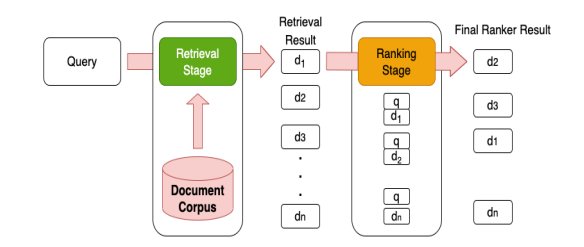
\includegraphics[width=14cm]{figs/chapter2/IR_system.png}
    \centering
    \caption{Overview of an interaction-based Information Retrieval model: Retrieval and Ranker.}
    \label{fig_ir_system}
\end{figure}

After analyzing the query, the retrieval stage will select an initial set of documents that are potentially pertinent to the query, as shown in figure \ref{fig_ir_system}. Subsequently, the relevance of these documents undergoes reassessment through the similarity scores. 

This is followed by the ranking stage, in which the primary objective is to adjust the order of the initially retrieved documents based on their relevance scores using a neural reranking, like {\bert} \cite{chen_integrating_2023}. This phase prioritizes the enhancement of result effectiveness rather than efficiency. In the end, it returns a rank of documents as close as possible to the user's query criteria. 


\subsection{Question Answering}

{\nlp} is the basis for building a {\qa} system, so it is important to give an overview of this technique. It is a field of {\ai} whose primary goal is to understand, interpret, and generate human language. The {\nlp} can be divided into two major components: {\nlu} and {\nlg}, according to \citet{ayanouz_smart_2020}

The \textbf{ {\nlu} } component is focused on enabling machines to understand and interpret human language in a meaningful way. {\nlu} involves processing and analyzing natural language data to comprehend its meaning, context, sentiment, and intent. 

In agreement with \citet{ngai_intelligent_2021}, the user queries can be processed by semantic analysis, pragmatic analysis, and syntactic analysis. \citet{ayanouz_smart_2020} explained these steps and added two more necessary steps to make it easier to understand: a lexical analysis and discourse integration.

\begin{itemize}
    \item \textbf{Lexical Analysis}: This step involves analyzing and identifying the structure of words. It breaks down the text into chapters, sentences, phrases, and words. \citet{chizhik_challenges_2020} defined lexical analysis as the pre-processing of the text following the steps: tokenization, removal of special characters, links, and punctuation, and removal of stop-words.

    \item \textbf{Syntactic Analysis}: The syntactic analyzer parses the grammar and arrangement of words, making the relationships between different words more explicit. Essentially, it rejects sentences with incorrect structures. This analysis can be seen as the process of normalizing tokens.

    \item \textbf{Semantic Analysis}: This step ensures the text is meaningful and interprets its correct meaning by mapping syntactic constructions. It ensures that only semantically valid content is retained. The recognition of entities is part of this analysis.

    \item \textbf{Pragmatic Analysis and Discourse Integration}: This step analyzes the overall context to derive the conclusive interpretation of the actual message in the text. It considers factors like the true meaning of a phrase or sentence based on the broader context.
\end{itemize}

The other component is \textbf{{\nlg}}. Language generation is responsible for crafting coherent and linguistically accurate responses. Simply put, it grapples with the challenge of navigating the intricacies of natural human language \cite{ngai_intelligent_2021}. 

Backtracking, {\qa} is a subfield of {\ir} and {\nlp}. According to \citet{zhong_building_2020}, {\qa} focuses on providing a single and specific answer to a question posed in natural language. Unlike {\ir}, which aims to return a broad range of relevant information or documents in response to a query, {\qa} seeks to pinpoint and provide one precise answer.

The traditional approach to question analysis and answering often involves mapping questions into predefined templates, such as "What-type" and "How-type". While widely utilized by existing online question-answering search engines, this template-based approach faces limitations in handling multiple questions \cite{zhong_building_2020}. 

So, with the advancement of technology, another approach emerged: deep learning-based question-answering. In contrast with the traditional approach, this approach employs deep learning techniques, like {\rnn}, to offer automatic representation and analysis of questions. These neural models, trained through end-to-end approaches, excel in extracting and understanding complex characteristics in textual documents.

Recently, deep learning approaches with attention mechanisms and transfer learning have enhanced the flexibility of representation in text classification and named entity recognition. \citet{zhong_building_2020} highlights {\bert} that has emerged as a powerful model, utilizing contextualized representations for transfer learning. {\bert}-based models showcase performance in question-answering tasks, even in domains like medicine.



\section{Large Language Models}
\label{llm}

It is crucial to trace briefly the development history to understand the concept of {\llm}. \citet{liu_prompting_nodate} explained this simply and intuitively.

Before {\llm}, there were only simple {\lm}, a subfield of {\nlp} and {\ai}, that have been called foundation models. A {\lm} is a statistical model used to predict the next word in a sequence of words. It calculates the probability of a given word occurring in a sequence, helping to determine which words are likely to appear next in a given context \cite{chang_language_2023}.

Most of these predictive models were based on probabilities and Markov assumptions, also known as {\slm}. This was heavily dependent on feature engineering. Afterward, as deep learning gained prominence, an architecture designed to learn data features automatically; in other words, neural networks for {\nlp} emerged to enhance {\lm}’s capabilities. Integrating feature learning and model training, {\nlm} established a comprehensive neural network framework applicable to diverse {\nlp} tasks \cite{liu_prompting_nodate}.

Most recently, the launch of the Transformer Block Architecture by \citet{vaswani_attention_2023} revolutionized this field. These deep-learning architectures led to the development of pre-trained models not explicitly designed for a particular task, including {\bert} and {\gpt}, collectively known as {\plm}. {\plm} have shown significant performance enhancements across various {\nlp} tasks.

Following this, the researchers have involved the scale of model parameters, and the paradigm of “Pre-train, Prompt, Predict" like \citet{liu_prompting_nodate} call, gained widespread acceptance. So, in terms of interaction with {\lm}, the prompts became crucial. Researchers name these {\plm} with hundreds of billions of parameters as {\llm}. Prompts effectively allow {\llm} to deal with a large number of complex and diverse tasks without a lot of effort.

This section discusses mainly {\llm}, exploring briefly their architecture and comparison between foundation {\llm}. Finally, it addresses some of its limitations.


\subsection{Definition}

{\llm} is an advanced {\lm} and belongs to generative {\ai}. It is designed to comprehend and generate text that is coherent and contextually relevant, engaging in human language interactions. Essentially, these advanced {\ai} systems mimic human intelligence. These models have a notable ability in natural language tasks, such as text generation and translation, {\qa}, decision-making, summarization, and sentiment analysis.

These models can process and predict patterns with accuracy. \citet{hadi_LLM_2023} combine sophisticated {\slm} and deep learning techniques to train, analyze, and understand huge volumes of data, learning the patterns and relationships among the data. For this reason, according to \citet{naveed_comprehensive_2023}, when provided with task descriptions and examples through prompts, {\llm} can produce textual responses to task queries. 

\citet{liu_prompting_nodate} say that the release of ChatGPT 1 garnered significant social attention, and research into {\llm} triggered more interest. This has led to the development of noteworthy products like PaLM, {\gpt}-2, {\gpt}-3, and, most recently, {\gpt}-4, and LLaMA and LLaMa-2.

{\llm} are revolutionizing {\nlp} and {\ai} research.


\subsection{Architecture Overview}

This subsection discusses the architecture of a {\llm}, which is supported by the Transformer Block architecture. Also, explains the pre-training process of this advanced {\lm}.

\subsubsection{Transformer Architecture}

The development and advancement of {\llm} is thankful for the introduction of Transformers by \citet{vaswani_attention_2023} in 2017. Most {\llm} are built on the Transformer model, which is based on a multihead self-attention mechanism and feedforward layers. This new technology enables parallelization and efficient handling of long-range dependencies, according to \citet{hadi_LLM_2023}, and led to the development of models that have achieved enormous results, such as {\gpt} by OpenAI and {\bert} by Google. The architecture of this revolutionized model is shown in figure \ref{fig_trans_arch}.

The innovation of this model is due to the multihead self-attention mechanism, one of the key components \cite{vaswani_attention_2023} \cite{hadi_LLM_2023}. It allows the model to weigh the importance of different words in a sequence when processing each word. This mechanism enables the model to focus on relevant information, capturing dependencies regardless of word order. 

However, the key advantage of this multihead self-attention mechanism is its highly parallelization \cite{vaswani_attention_2023}. This characteristic enables the Transformer model to be easily distributed and trained on a large scale using GPUs. The ability to parallelize computations means that Transformers can handle larger datasets and more complex tasks, unlike previous architectures like {\rnn}, where sequential processing of data was required.

Since the model doesn't have recurrence and convolution to understand the order of the input sequence, another component, Position Encoding, provides some information about the position of the tokens in the sequence. This is crucial for capturing sequential information in the data. 

\begin{figure}[ht]
    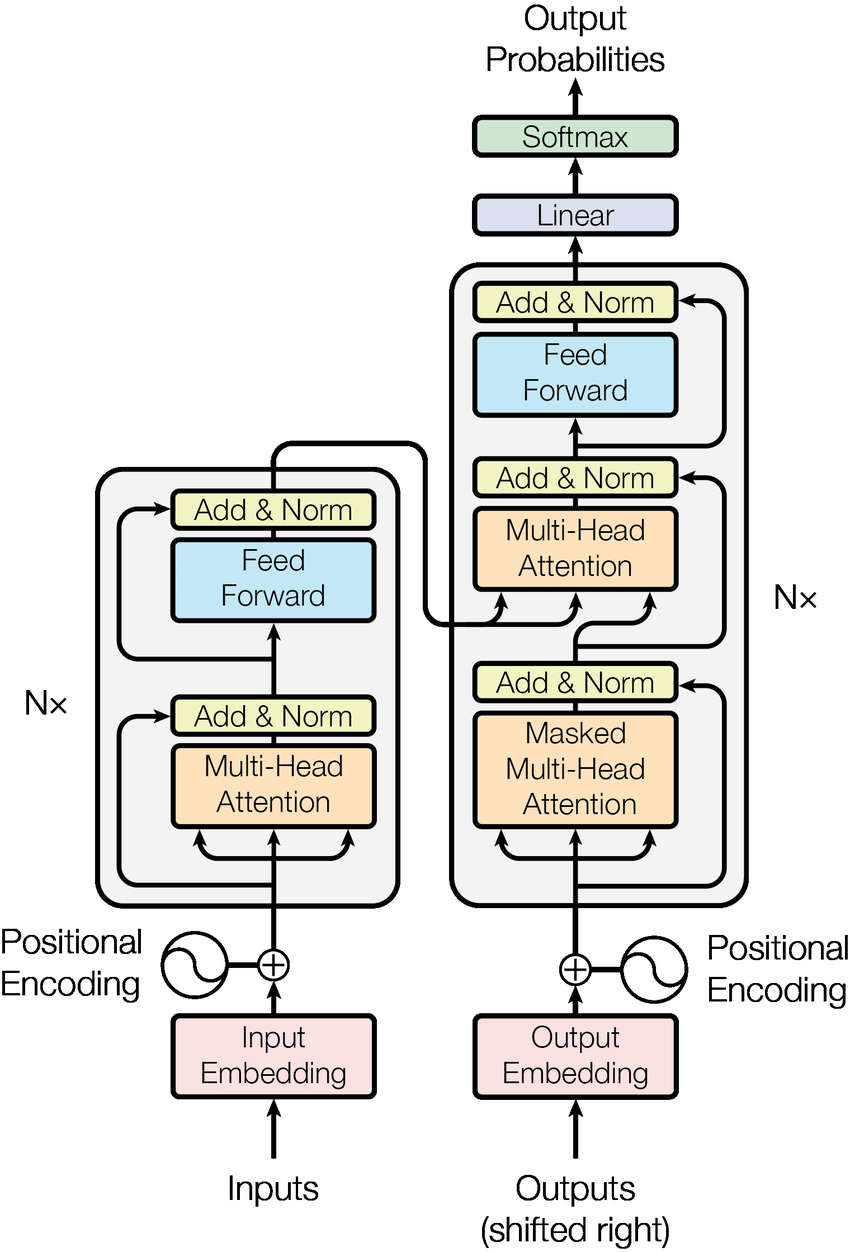
\includegraphics[width=8cm]{figs/chapter2/transformer.png}
    \centering
    \caption{The Transformer Block Architecture, from \citet{vaswani_attention_2023}.}
    \label{fig_trans_arch}
\end{figure}


\subsubsection{Pre-training Process}

Learning the patterns and relationships among the data starts with the pre-training process. In compliance with \citet{min_recent_pretrained}, first, the {\llm} needs to access a vast volume of textual data from multiple sources. The goal of this phase is to predict the succeeding word in a sentence based on the context given by the previous words through unsupervised learning. 

According to \citet{hadi_LLM_2023}, preparing and preprocessing the data before the training stage is necessary to achieve this. First, demand quality filtering from the training corpus. It is vital to remove unwanted, repetitive, duplicated, superfluous, and potentially harmful content from the massive text data. Next, it is necessary to pay attention to privacy. The data could have sensitive or personal information, so it is vital to address privacy concerns by removing this information from the pre-training corpus.

An important step, the tokenization, follows this \cite{hadi_LLM_2023}. This step aims to divide the unprocessed text into sequences of individual tokens, which are subsequently input into {\llm}. Moreover, it is vital in mitigating the computational load and enhancing efficiency during the pre-training phase. Figure \ref{fig_tokenization} visually presents the tokenization process \cite{noauthor_openai_nodate} carried out and explained by OpenAI.

\begin{figure}[ht]
    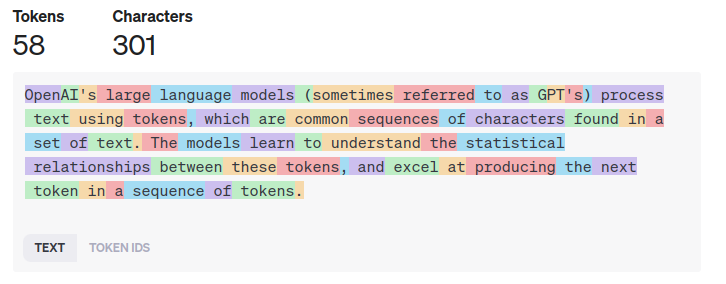
\includegraphics[width=14cm]{figs/chapter2/tokenization.png}
    \centering
    \caption{Tokenization process visually explained by OpenAI \cite{noauthor_openai_nodate}.}
    \label{fig_tokenization}
\end{figure}

After the pre-training process, the {\llm} goes through an optimization phase.


\subsection{Optimization Techniques}

There are some techniques to optimize the tasks and the accuracy of the {\llm}. Two of these techniques, Fine-tuning and Prompt Engineering, are explained next.


\subsubsection{Fine-tuning}

During pre-training, models are generally trained with the objective of next token prediction, learning the nuances of language structure and semantics. According to \citet{kamnis_generative_2023} and \citet{hadi_LLM_2023}, the fine-tuning phase involves adapting a pre-trained model to specific tasks and aligning it with human preferences, improving the performance on particular domains.

In this stage, the model is presented with labeled data to produce more contextually accurate responses for the specific task. Fine-tuning enables the {\llm} to specialize in diverse applications, ranging from language translation and question-answering to text generation. 

Some approaches could be applied to fine-tune the model. \citet{naveed_comprehensive_2023} distinguishes some of them, such as Parameter-Efficient Tuning. As {\llm} typically requires a lot of computational resources, like memory and computing, the Parameter-Efficient Tuning approach is helpful because it allows the model to train by updating fewer parameters, adding new ones, or selecting existing ones. Inside this approach, there are also some different methods. The commonly used indicated by \citet{naveed_comprehensive_2023} are Prompt Tuning, Prefix Tuning, and Adapter Tuning.

The Prompt Tuning method integrates trainable tokens, named soft prompts, to the beginning or within the input of a {\llm}, and only these tokens are adjusted during training to adapt the model for a specific task. This method keeps the rest of the model unchanged, ensuring the core knowledge and capabilities of the model are preserved while it learns to handle new types of requests or information.

In Prefix Tuning, a sequence of trainable tokens is introduced to transformer layers, with only the prefix parameters undergoing fine-tuning, while the remaining model parameters remain unchanged. These added prefixes function as virtual tokens, allowing input sequence tokens to attend to them during processing.

Meanwhile, in Adapter Tuning, small modules called adapters are added inside each layer of the Transformer. These adapters can be trained to adapt the model for specific tasks. The fine-tuning process works by slightly altering the model's internal features, allowing it to learn task-specific patterns without changing the entire model. LoRA (Low-Rank Adaptation) is one technique that implements Adapter Tuning, introduced by \citet{hu_lora_2021}. Instead of adding new layers like traditional adapters, LoRA learns low-rank matrices that are used to update the weights of the existing layers, maintaining the original weights of the model. This approach allows for efficient fine-tuning of the model on specific tasks while maintaining the model's original performance and avoiding significant increases in computational costs.


\subsubsection{Prompt Engineering}

With the emergence of {\llm}, other research fields were born. Prompt Engineering is one of these cases and has been widely applied. In compliance with \citet{mesko_prompt_2023} and \citet{ma_beyond_2023}, this emerging field involves designing, refining, and implementing prompts or instructions to direct the generated output of {\llm}, aiding in diverse tasks. {\llm} can follow specific directions provided by users in natural language after being tuned with instructions.

There are some techniques of prompt engineering, such as Chain of Thought (CoT) and Reason-Action (ReAct). 

CoT is a popular problem-solving approach for prompt engineering that aims to break complex tasks into multiple and simpler subtasks and solve them. So, \citet{wei_chain--thought_2023} explained that this method involves explicitly modeling the reasoning processes that lead to a final answer, rather than directly generating an answer. This explanation of reasoning often leads to more accurate results. Figure \ref{fig_cot} explains the effect of this technique.

ReAct is a prompt technique introduced by \citet{yao_react_2023}. The idea behind this is to simultaneously include both reasoning and action within a single prompt. To solve a complex task, ReAct consists of three tasks for every subtask: 1) \textbf{Reason} involves analyzing the current situation and determining the necessary steps; then, 2) \textbf{Action} entails executing a task based on the reasoning. 3) \textbf{Observation} then refers to examining the outcomes following the action.


\begin{figure}[ht]
    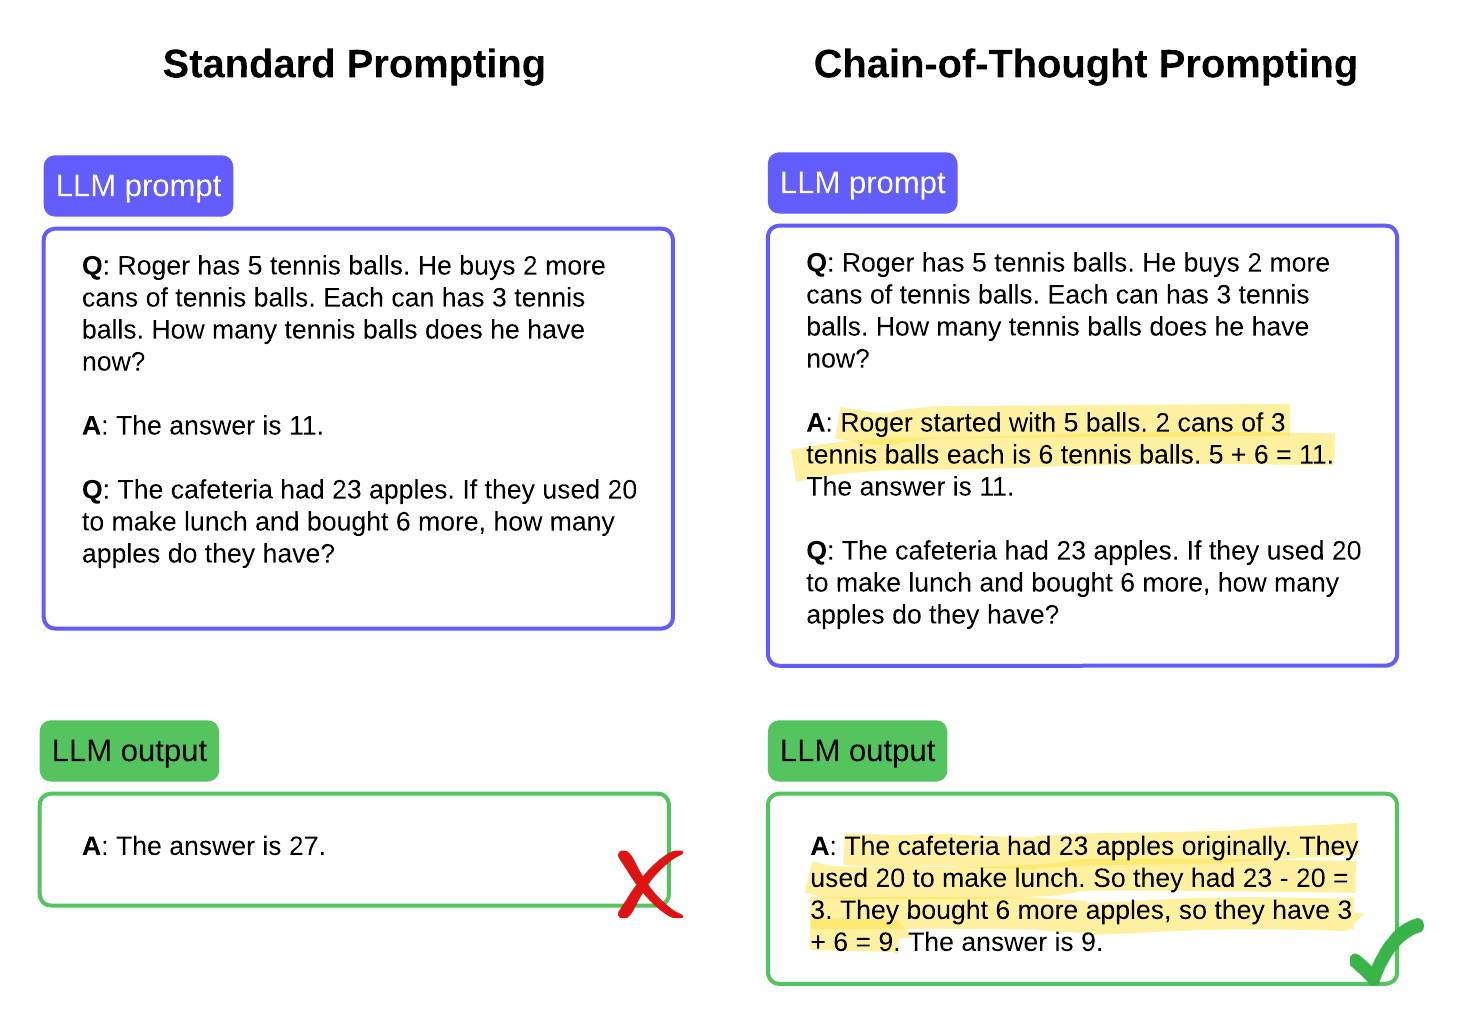
\includegraphics[width=14cm]{figs/chapter2/CoT.png}
    \centering
    \caption{Example of Chain-of-thought prompting. The reasoning processes are highlighted in yellow. Adapted from \citet{wei_chain--thought_2023}.}
    \label{fig_cot}
\end{figure}


\citet{mesko_prompt_2023} raise a series of recommendations for more effective {\llm} prompts: it must be as precise as possible; providing the setting and the context of the question is essential; describe the goal of the prompt first; give a role to the {\llm} to get more context (for example, "You are a math teacher and explain the natural numbers"); continuous {\llm} prompt refinement; prefer open questions over close-questions. Regularly testing prompts in real-world situations is crucial, as their effectiveness is most accurately assessed through practical application.



\subsection{Comparison between foundation Large Language Models}

The best way to compare {\llm} is to evaluate the model's performance. \citet{hadi_LLM_2023} identified five factors to make this comparison: the size of the training corpus, the quality of the training corpus, the number of parameters, the complexity of the model, and some test tasks.

The primary foundation models of {\llm} are {\gpt}-4 by OpenAI, LLaMA 2 by Meta, PaLM 2 by Google, and Falcon by Technology Innovation Institute (TII). These {\llm} are provided by big companies and have outstanding progress in the evolution of this area. These models gave rise to many others.

LLama 2 is an open source {\llm} by Meta (\citet{touvron_llama_2023}). LLaMa 2 was trained on 40\% more data than LLaMa 1, the model from which it came, and has double the context length. So, the model size of LLaMa 2 is 7 billion, 13 billion, or 70 billion parameters. With 4096 context length and trained on 2 trillion pretraining tokens, this {\llm} is commonly fine-tuned for chat use cases. Many other models, like Alpaca, Vicuna, and Llama-2-chat, came from LLaMa and deserve further analysis. It is accessible for both research and commercial purposes

The recent {\gpt} model from OpenAI, {\gpt}-4, is a closed source {\llm} (\citet{openai_gpt-4_2023}). Trained on a meticulously curated dataset from various textual sources, including books, articles, and websites, {\gpt}-4 exhibits remarkable performance with text and image inputs. It is the {\llm} behind ChatGPT. It has 32 000 context length. OpenAI has chosen to provide limited technical details about the training methodology used for this advanced model, including specific information on parameter counts.

The Google generative chatbot, Bard, uses as {\llm} the PaLM 2 model developed by Google (\citet{anil_palm_2023}). It emerged from PaLM with 540 billion parameters. PaLM 2 is a closed source {\llm}, and, following the OpenAI approach, has opted to disclose limited technical specifics, including the number of parameters. 

The Falcon {\llm} is an open-source model with impressive performance and scalability (\citet{almazrouei_falcon_2023}). There are three variations of the model size: 7 billion, 40 billion, and the most recent, 180 billion of parameters. This Falcon 180B is equipped with an impressive 180 billion parameters and trained on 3.5 trillion tokens. It is accessible for both research and commercial purposes.

The table \ref{table:comparison} summarizes the important aspects of comparison between this foundation {\llm}.

\begin{table}[ht]
    \scalebox{0.8}{
        \begin{tabular}{|c|c|c|c|c|c|c|}
        \hline
        \textbf{Model} & \textbf{Provider} & \textbf{\begin{tabular}[c]{@{}c@{}}Model size\\ (Parameters)\end{tabular}} & \textbf{Context Length} & \textbf{Tokens} & \textbf{Fine-tuneability} & \textbf{Open-source} \\ \hline
        GPT-4          & OpenAI            & -                                                                          & -                       & -               & No                        & No                   \\ \hline
        LLaMa 2        & Meta              & 7B, 13B, 70B                                                               & 4096                    & 2T              & Yes                       & Yes                  \\ \hline
        PaLM 2         & Google            & -                                                                          & -                       & -               & No                        & No                   \\ \hline
        Falcon         & TII               & 7B, 40B, 180B                                                              & 2048                    & 3.5T            & Yes                       & Yes                  \\ \hline
        \end{tabular}
    }
    \caption{Comparison of foundation Large Language Models.}
    \label{table:comparison}
\end{table}



\subsection{Limitations}

It is safe to say that {\llm} are significantly impacting the world. According to \citet{liu_prompting_nodate}, this is justified by their abilities, mainly in-context learning, reasoning for complex content, instruction following, and creative capacity.

However, {\llm} has some limitations. \citet{hadi_LLM_2023} address some of them, and the most important ones are biased responses, hallucination, explainability, and cyber-attacks. 

We already know that {\llm} are pre-trained with extensive training data. But suppose that data contains some biased information related to factors such as gender, socioeconomic status, and/or race. In that case, this may result in analyses and recommendations that are discriminatory or inaccurate across diverse domains. The problem of bias applies not only to training data but also to user interaction bias, algorithmic bias, and contextual bias. The user interaction bias means that, as user prompts shape responses, and if users consistently ask biased or prejudiced questions, the model may acquire and reinforce these biases in its replies.

A severe limitation that is an active area of research is hallucination. \citet{church_emerging_2023} characterized {\llm} hallucinations as when the model attempts to fill gaps in knowledge or context, relying on learned patterns during training. Such occurrences can result in inaccurate or misleading responses, detrimental to the user and the model's reliability.

The way the {\llm} makes decisions is unknown. Comprehending the decision-making process of a complex model with billions of parameters, like {\llm}, is challenging. So, the explainability of these models is a big limitation \cite{hadi_LLM_2023}. Sometimes, it is necessary to decipher the factors that influenced an {\llm}'s decision and this limitation poses difficulties in offering a clear and concise explanation. In vital sectors like healthcare, where decisions carry substantial consequences, ensuring transparency and the capability to elucidate the model's predictions is essential.

Another limitation is the cyber-attacks. A {\llm} can suffer some prompt injections from a malicious user to extract sensitive information from the model, according to \citet{kshetri_cybercrime_2023}. This is called the Jail Break attack \cite{hadi_LLM_2023}. Another attack is Data Poisoning Attacks, which consist of data poisoning strategies to manipulate the model's output.

Furthermore, \citet{liu_prompting_nodate} highlighted another limitation: the temporal lag of the training corpus. {\llm} cannot retrieve information in real time, and the answer generated may not be the most current.

It is important to be aware of these limitations.


\section{Conversational User Assistants}

Conversational User Assistants, also known as chatbots, chatterbots, or virtual assistants, have become a vital aspect of the digital landscape. These tools are generally dialogue systems that understand, interpret, and generate human language, enabling them to communicate with users to dissolve their questions.

Chatbots are increasingly being used in various contexts due to their many benefits. These aspects that make companies bet on the use of chatbots are the continuous availability to support and assist the customer, ensuring more consistent support; the cost-efficiency by reducing the human customer support; the time-saving both for the organization and for customers due to the immediate responses to the user queries; the ease and intuitiveness of this systems; and, improve service with every interaction \cite{misischia_chatbots_2022}. Because of this, the utility of the chatbots as tools is increasing as the technology advances. 

The rise of conversational user assistants is underpinned by a convergence of technologies, specifically by {\llm}.

This section provides a brief overview of chatbots, followed by an in-depth focus on Generative-Based Chatbots. It encompasses important concepts from their definition to some techniques employed in their development and optimization.


\subsection{Overview of Conversational User Assistants}

To provide a comprehensive understanding of conversational user assistants, it's crucial to first explore some of their characteristics, such as domains and method of response generation.

\citet{nuruzzaman_survey_2018} defined the differences between chatbots with opened or closed domains. In an open-domain environment, conversations can go in any direction without a predefined goal or intention. Conversely, in closed-domain environments, the conversation is centered on a particular topic. A closed-domain chatbot is designed with a clear objective.

It is important to differentiate chatbots in their way of giving or generating a response based on an input query. \citet{peng_survey_2019} distinguish three main types of chatbots based on their response generation: Rule-based, Retrieval-based and Generative-based chatbots.

A \textbf{rule-based chatbot} examines fundamental features of the user's input statement and generates a response based on a predefined set of manually crafted templates. This type is more applicable in a closed-domain conversation. ELIZA, introduced by \citet{weizenbaum_elizacomputer_1966}, was the first chatbot that applied this primitive technique.

A \textbf{retrieval-based chatbot} picks a response from an extensive precompiled dataset. It selects the most promising reply from the top-k ranked candidates. Thus, they refrain from producing new text. It has limited flexibility regarding closed-domain and in terms of errors \cite{agarwal_review_2020}.

A \textbf{generative-based chatbot} generates a text sequence as a response rather than choosing it from a predefined set of candidates. These chatbots are very flexible and can handle open domains because they are implemented with deep learning techniques. The interactions will be more identical to those of humans, as it implements a self-learning method from a large quantity of interaction data \cite{peng_survey_2019} \cite{agarwal_review_2020}. However, this could be complex and costly to implement.

The only type that will be covered will be generative chatbots, due to their capabilities.


\subsection{Generative-Based Chatbot}

Generative-based conversational user assistants are chatbots that use generative models to generate natural language responses. These chatbots utilize sophisticated deep-learning techniques, such as {\llm}. {\llm}, as described in section \ref{llm}, has the ability to understand and generate human-like text in context. This advanced {\lm} has been widely used in the modern chatbots. ChatGPT is an example of this type of chatbot.

Although an {\llm} can generate text from a query, it is not prepared to be applied to a chatbot. There are some techniques for improving and optimizing the model to behave like a chatbot, such as {\rlhf}.

In addition, some techniques aim to combat some of the limitations of chatbots, such as hallucination, by increasing their knowledge, such as {\rag}.

The {\rlhf} and {\rag} are explained in more depth below.


%%%%%%%%%%%%%%%%%%%%%%%%%%%%%%%%%%%%%%%%% commented %%%%%%%%%%%%%%%%%%%%%%%%%%%%%%%%%%%%%%%%%
\iffalse       

There are some methods to improve the results of a {\llm} used on chatbot: fine-tuning the {\llm}, {\rag}, and Prompt Engineering.

\begin{table}[ht]
    \centering
    \begin{tabular}{|cc|cc|}
    \hline
    \multicolumn{2}{|c|}{\multirow{2}{*}{\textbf{}}}                                                                                 & \multicolumn{2}{c|}{\textbf{Model Adaptation Required}}                                                                   \\ \cline{3-4} 
    \multicolumn{2}{|c|}{}                                                                                                           & \multicolumn{1}{c|}{Low}                                                                             & High               \\ \hline
    \multicolumn{1}{|c|}{\multirow{2}{*}{\textbf{\begin{tabular}[c]{@{}c@{}}External \\ Knowledge \\ Required\end{tabular}}}} & Low  & \multicolumn{1}{c|}{Prompt Engineering}                                                              & Fine-tuning        \\ \cline{2-4} 
    \multicolumn{1}{|c|}{}                                                                                                    & High & \multicolumn{1}{c|}{\begin{tabular}[c]{@{}c@{}}Retrieval-Augmented \\ Generation (RAG)\end{tabular}} & All of the methods \\ \hline
    \end{tabular}
    \caption{Optimization methods of generative-based chatbots.}
    \label{table:optimization}
\end{table}

The table \ref{table:optimization} shows how these methods influence model adaptation and external knowledge. Mixing all methods requires a high model adaptation and external knowledge, but provides better results. 

\fi
%%%%%%%%%%%%%%%%%%%%%%%%%%%%%%%%%%%%%%%%% commented %%%%%%%%%%%%%%%%%%%%%%%%%%%%%%%%%%%%%%%%%


\subsubsection{Reinforcement Learning from Human Feedback (RLHF)}

In the context of {\ai}, according to \citet{li_human-centered_2019}, {\rlhf} is a popular approach in which an agent learns how to perform a task based on evaluative feedback provided by a human observer.

{\rlhf} in generative-based chatbots is a topic that has been explored in the field of conversational {\ai}. This technique is a transformative technique that combines reinforcement learning and supervised learning to refine {\llm} for chatbot applications. \citet{tran_enhancing_2023} stated that {\rlhf} aims to align chatbot responses to human preferences, improving chatbots' performance and making them more human-like.

The process encompasses several crucial stages, in conformity with \citet{axelsson_modeling_2022}. Initially, the {\llm} is pre-trained on a large dataset of text, which allows it to learn a wide range of language patterns and knowledge. After pre-training, the model undergoes a phase of supervised fine-tuning. In this phase, the {\llm} is trained on a dataset of conversational examples that are specifically curated to reflect the desired outputs for the chatbot. 

After that, humans provide feedback on the model's outputs. This feedback is crucial because it is used to build and train a reward model. The reward model learns to predict the quality of the model's responses based on the human-provided feedback \cite{axelsson_modeling_2022}.

The {\llm} is further fine-tuned using reinforcement learning, where it learns to generate responses that maximize the predicted reward, using the reward model created in the previous phase. This stage enables the model to optimize its responses through the reward model, which is based on human feedback.

The process often involves several iterations of feedback and fine-tuning to continually improve the chatbot's performance. This can resolve errors, improving the refining the conversational style.



\subsubsection{Retrieval-Augmented Generation (RAG)}

{\rag} is a subfield of {\nlp} and {\ai}. This approach was introduced by \citet{lewis_retrieval-augmented_2020} in 2020 and combines retrieval-based and generative models to enhance content generation and information retrieval processes. For a clearer comprehension of this method, \citet{gao_retrieval-augmented_2023} made a survey into {\rag} systems and distinguish the parametric knowledge from non-parametric knowledge. 

Traditionally, {\llm} can adapt their knowledge and responses to a specific domain by fine-tuning models with parameters. This is \textbf{parametric knowledge} because the {\llm} knowledge is provided through the model's training data. However, entirely parameterized {\llm} have limitations, including data not currently updated and hallucinations. The \textbf{non-parametric knowledge}, provided by external information sources, emerged to solve these limitations. This non-parametric knowledge approach is known as {\rag}. 

So, according to \citet{lewis_retrieval-augmented_2020}, {\rag} involves retrieving pertinent information from external knowledge bases, giving more context to the {\llm}. This enables the {\llm} to access and utilize up-to-date and/or domain-specific information to enhance response accuracy and relevance. This process leads to reducing hallucinations.

The figure \ref{fig_rag} shows the workflow of a {\rag}. This model aims to retrieve relevant information from an extensive corpus of documents when answering questions, subsequently adding this information in the prompt as context to enhance the quality of predictions in compliance with \citet{lewis_retrieval-augmented_2020}.

%% FIXAR ESTA IMAGEM
% image reference: https://towardsdatascience.com/retrieval-augmented-generation-rag-from-theory-to-langchain-implementation-4e9bd5f6a4f2
\begin{figure}[ht]
    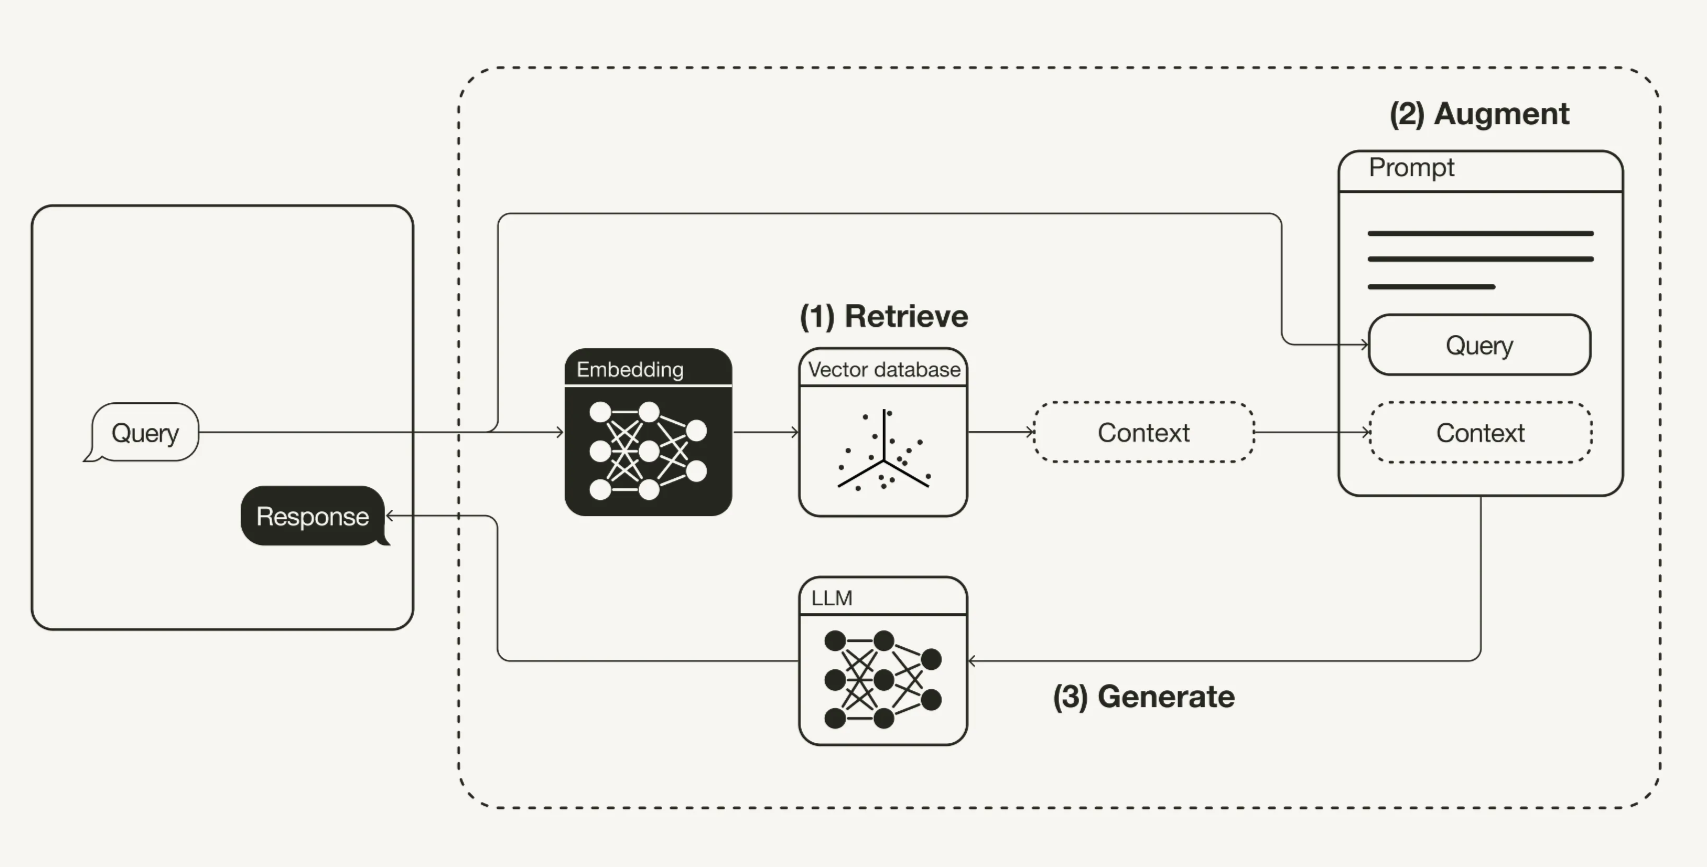
\includegraphics[width=14cm]{figs/chapter2/rag_workflow.png}
    \centering
    \caption{Retrieval-Augmented Generation Workflow.}
    \label{fig_rag}
\end{figure}


\citet{gao_retrieval-augmented_2023} explain simply the workflow. The first step is 1) Retrieve information from an external data source, such as a vector database, as in the example in figure \ref{fig_rag}. This step utilizes {\ir} models, such as {\bm}, to retrieve relevant information based on the query. The second step is 2) Augment, improving the {\llm} prompt with the context retrieved in the previous stage. The last step is 3) Generation. Using the prompt with context, the {\llm} generates a response to the query, based on the external information retrieved.

% escrever mais? vantagens,  RAG vs Fine-tuning, tipos de RAG


\section{Interactive Query Builder}

A query builder is a user interface tool for dynamically searching and filtering database objects, constructing a query according to user preferences, as the work of \citet{mussa_forestqb_2022} shows. This query could be in different formats, such as SQL and JSON. This tool lets users construct queries visually, eliminating manual research or coding. 

This section is particularly significant as there is limited documentation on conversational query builders. Therefore, it documents the general workings of query builders and delves into a detailed explanation of the functioning of the ATLAS cohort definition.

\subsection{General Query Builders}

% explicar como funcionam de forma geral

Users interact with the query builder through a user-friendly interface. Figure \ref{fig_query_builder} shows a query builder interface from jQuery QueryBuilder \cite{noauthor_jquery_nodate}.

\begin{figure}[ht]
    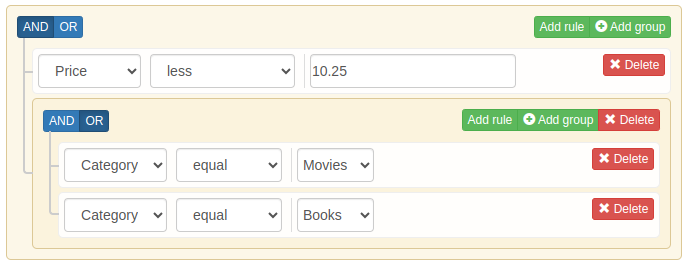
\includegraphics[width=14cm]{figs/chapter2/querybuilder.png}
    \centering
    \caption{Query builder from jQuery QueryBuilder \cite{noauthor_jquery_nodate}.}
    \label{fig_query_builder}
\end{figure}

Users can add rules and conditions/groups with some clicks. Each rule typically consists of a field, an operator, and a value. The conditions/groups could be an AND or an OR. Using figure \ref{fig_query_builder} as an example, there is a group with two elements joined with a condition AND: a rule and another group. This other group is composed of two rules joined with a condition OR.

As users build their queries, the query builder internally represents the conditions in a structured format, often a structured JSON of rules and groups, that reflects the logical structure of the query \cite{noauthor_jquery_nodate}.

In summary, a query builder simplifies creating complex queries by providing a visual and interactive interface, making it more accessible \cite{noauthor_introducing_2021}.

There are several advantages of its use \cite{noauthor_introducing_2021}: offers a user-friendly interface with menus, operators, and suggestions to facilitate the creation of accurate queries; users, often without direct permissions to modify the data source, can leverage the query builder to transform datasets without making changes to the underlying database; and, the generated queries are easily modifiable, allowing for flexibility in adjustments or repetitions.


\subsection{ATLAS}

% explicar como funciona o processo

ATLAS, an open-source and web-based software application, is freely accessible and was created by the {\ohdsi} community. It aids in helping researchers conduct scientific analyses on standardized observational data converted to the {\omop}.

Using healthcare claims data, researchers can define cohorts by categorizing groups of people according to their exposure to a medication or their diagnosis of a certain health condition. ATLAS offers the functionality to search medical concepts, enabling the identification of cases with particular conditions or drug exposures. Moreover, it allows for the examination of patient profiles within a given cohort, providing a way to visualize the healthcare records of specific subjects.

There are some different definitions of cohort, but, in the {\ohdsi} research, according to \citet{informatics_chapter_nodate}, a cohort is a query that defines a set of persons who meet certain inclusion criteria over a specified duration.

Cohorts serve as fundamental units for addressing research questions. A key characteristic of these cohorts is their independent definition. The distinct structure facilitates their reuse across different research contexts.


\subsubsection{Cohort definition}

There are two approaches to building a cohort: rule-based and probabilistic. The most popular one is the rule-based cohort definition, which uses explicit rules to describe when a patient is in the cohort.

In ATLAS, the process of defining a cohort is composed of 3 stages \cite{informatics_chapter_nodate}: Cohort Entry Events, Inclusion Criteria, and Cohort Exit.

The creation of a cohort starts with \textbf{Cohort Entry Events}, defining the initial event criteria. This involves the primary identification of the population of interest, which might include users of a certain drug, individuals with a specific diagnosis, or a combination of factors. 

The concept set needs to be specified in the Cohort Entry Events. It is a collection of standardized medical concepts used to define clinical elements like diseases, drugs, or procedures. For instance, if the study is about diabetes, the concept set will include various codes representing diabetes in different medical terminologies. These sets ensure that the cohort captures all relevant instances of the condition or exposure across different healthcare data sources.

Additional initial event criteria can also be added to refine the population further, such as the event occurring within a certain time frame.

After defining the initial event, the next step is to establish \textbf{Inclusion Criteria}. These criteria are based on a combination of domain-specific attributes to further refine and specify the cohort population, ensuring that it aligns closely with the research objectives. The inclusion criteria can be based on a range of factors such as age limits, the presence of certain symptoms, or a specified duration of medication use.

Finally, defining the \textbf{Cohort Exit} criteria is crucial for determining when individuals no longer belong to the cohort. This stage is important for studies where the duration of membership in the cohort is relevant to the research question.

In compliance with \citet{informatics_chapter_nodate}, a well-defined cohort specifies how a patient enters a cohort and how a patient exits a cohort.

After defining the cohort, it is possible to generate an SQL code with the query to get the list of individuals who meet the criteria. ATLAS also facilitates the reuse of cohort definitions across different studies by allowing users to export and import cohort definitions in JSON format. This enhances the efficiency and reproducibility of research within the OHDSI network.

A cohort definition can be seen as a query builder, a little different when compared to other general query builders.

% meter uma imagem da interface ?


\section{Summary}

To sum up, the proposed query builder is a generative-based chatbot with a closed domain. Closed-domain chatbots are specialized in specific areas, offering precise responses. Generative chatbots use advanced {\lm} to create dynamic responses closer to human interactions.

The utilization of {\llm} allows improvements in the {\nlg} capabilities of chatbots and guides conversations more effectively, especially in the task of defining cohorts in medical research. LLaMa-2 and Falcon appear to be good options to implement since they are open-source and have the possibility of fine-tuning the model. Fine-tune has the role of optimizing chatbot performance, alongside Prompt engineering and {\rag}. However, for this specific case, I don't think much external knowledge will be needed, so the use of fine-tuning should be enough.

In terms of {\ir}, in order to retrieve the most interesting databases according to the user's needs, the {\bm} technique proves to be a good balance between effectiveness and efficiency. {\bm} is a sophisticated yet relatively straightforward algorithm that improves upon the traditional {\tfidf} approach. Neural {\ir} systems, like Interaction-based models, show good results in the {\ir} tasks, but are complex and the neural networks require substantial computational power. It is a lot simpler to implement than the Neural {\ir} systems, as well as requires fewer computer resources. 

ATLAS by OHDSI provides a cohort definition, which is a query builder to define groups of people based on the research question using healthcare claims data. However, the interface revealed not very user-friendly and intuitive because it requires the user to have a good knowledge of its use and important concepts. Therefore, a chatbot that builds a cohort definition improves the user experience by making it more intuitive and autonomous.


%  meter mais referencias e citações
\chapter{Methodology}
\label{chapter:Methodology}

For this thesis work, after an extensive literature review on crucial fields, concepts and technologies, we are ready to achieve the primary goal of this work.

This section presents the methodology applied to this project, from the work done to the work plan.

\section{Work Done}

This semester's work was mainly focused on state-of-the-art understanding and writing, going through a process of research and reading articles. The state-of-the-art objectives established in \autoref{chapter:Introduction} have been completed. These objectives are to study methodologies to build a conversational user interface, procedures to retrieve the databases of most interest and explore the definition of a study protocol. It was essential not only to learn more about the actual state of some technologies and concepts but also to get more into the project goal and requirements.

In terms of development, first, I built a prototype of an architecture, which is shown in figure \ref{fig_arch}, and then started the development.

\begin{figure}[ht]
    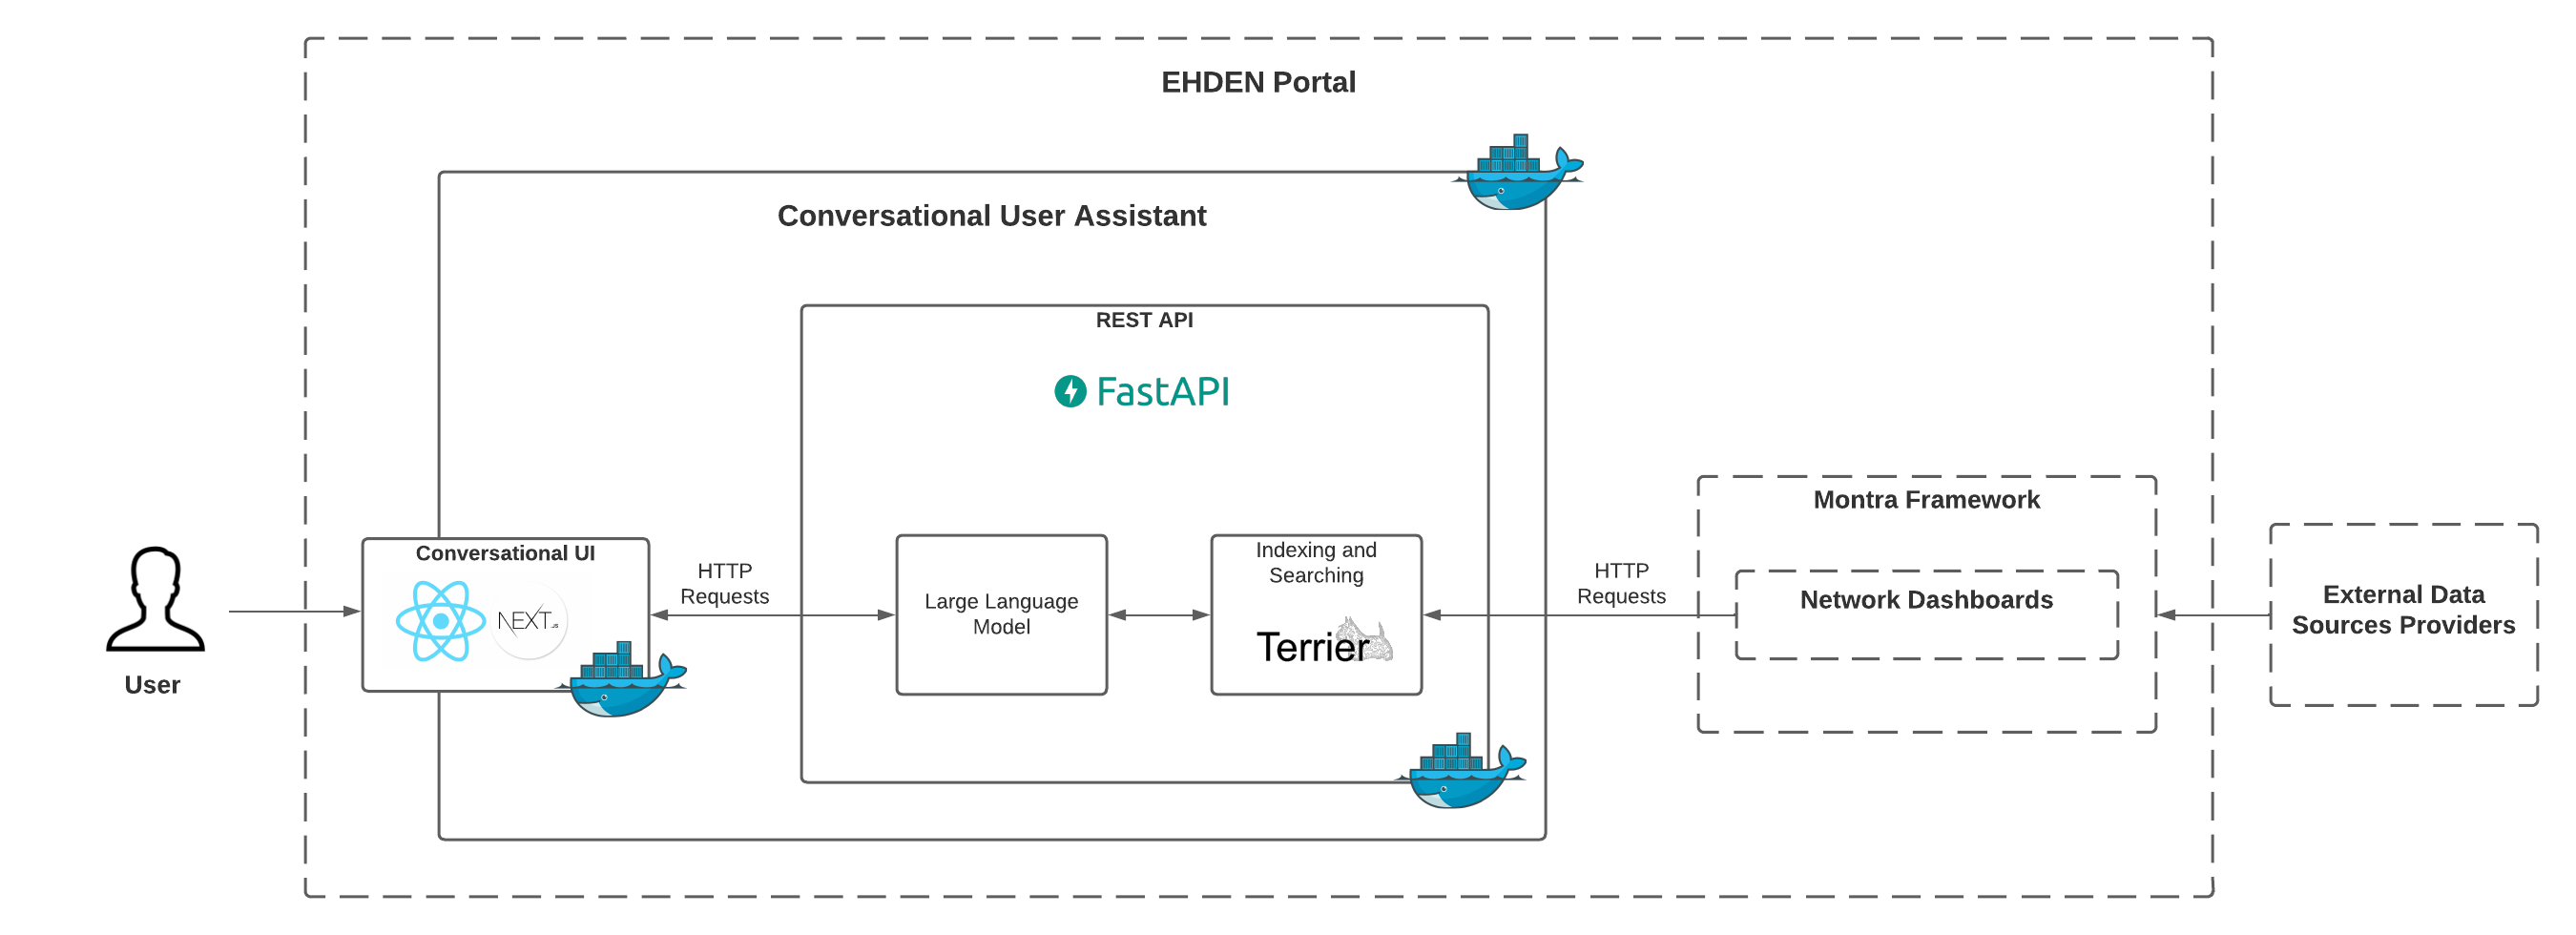
\includegraphics[width=16cm]{figs/chapter3/arquitetura.png}
    \centering
    \caption{Architecture Proposal. Only the components with a solid line relate to the proposed work.}
    \label{fig_arch}
\end{figure}

I have developed a prototype of a chat-like interface using NextJS, a well-known ReactJS framework. Also, I have developed a REST API in FastAPI, a modern web framework based on Python. The interface and the API communicate between them through HTTP requests. The components of this application are deployed in Docker containers.

Beyond this, inside the backend module, I have started implementing and testing a {\bm} method to retrieve the best databases for a given user query. First, {\nlp} methods are applied to understand the plain-text query. For now, the {\nlp} method is in a very simple stage, because only tokenization, normalization, stemming and lemmatization are applied. Then, the {\bm} score is calculated between the query and the concepts of which database, making a database ranking. To implement the {\ir} technique, I am using the pyterrier library, and it could be changed to another library later if I discover another one more effective. The PyTerrier library facilitates the creation of a collection, allowing for the indexing and searching of data using a {\bm} method.
 
So, for now, the application developed can receive a user query through the frontend module and then, the backend module retrieves a rank of databases based on the query understanding. The chatbot interaction with the user is limited, as shown in figure \ref{fig_interface}. When the chatbot identifies a concept, he retrieves a list of clickable buttons of the ranked databases, indicating the database ID and its {\bm25} score. However, if it doesn't, it sends a pre-defined message.

\begin{figure}[ht]
    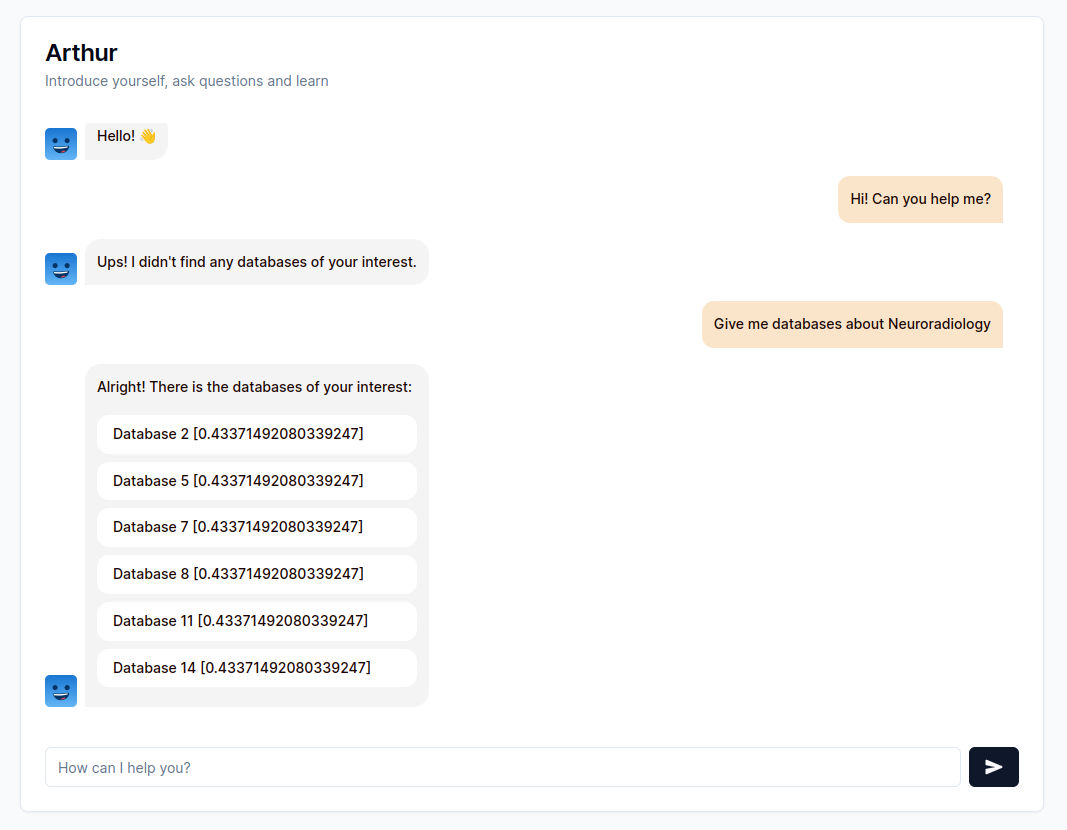
\includegraphics[width=12cm]{figs/chapter3/interface.png}
    \centering
    \caption{Example of an interaction with the chatbot, showing the current state of the project.}
    \label{fig_interface}
\end{figure}



\section{Future work}

For the following months, I will continue the development of the database recommendation, based on {\bm}, improving some aspects, like concept linking. Also, test and improve this {\ir} implementation based on the testing results. 

After this, I will choose, implement, and fine-tune a {\llm} in order to guide the conversation to build the final query with the cohort definition structure. By doing this, the conversation flows naturally. Finally, test and improve the model based on the testing results.

The next step is integrating this system in the {\ehden} Portal and testing and validating the system. 

The documentation of the implementation and the respective steps taken will be carried out throughout its development.

The subsection \ref{workplan} presents a plan for all these tasks.


\section{Work Plan}
\label{workplan}

The following Gantt diagram, figure \ref{fig_gantt}, shows the work proposal for the following months. This diagram is divided into two semesters: the first refers to the work done in the first semester, and the second to the work proposed for the second semester.

\begin{figure}[ht]
    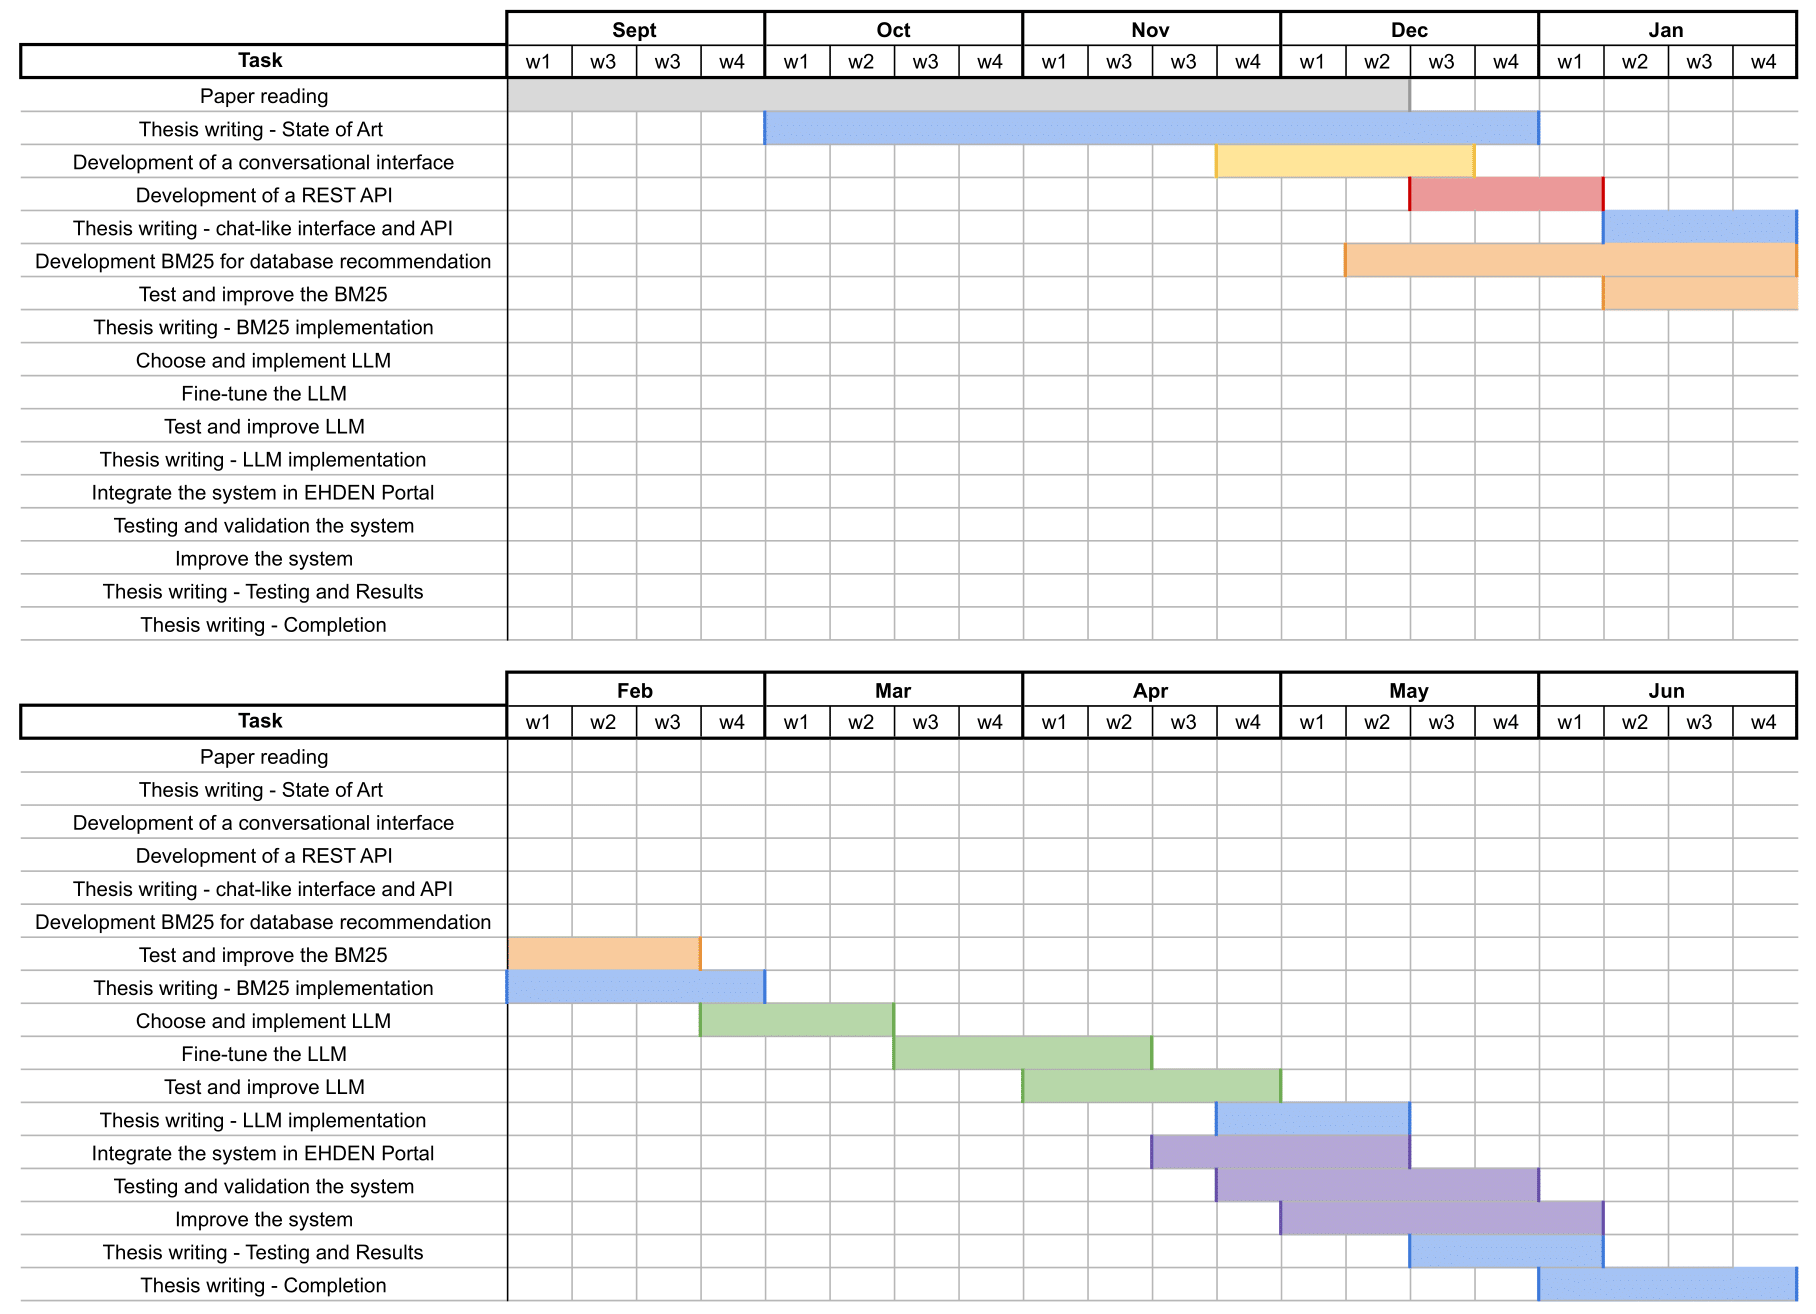
\includegraphics[width=16cm]{figs/chapter3/diagram_gantt.png}
    \centering
    \caption{Proposal thesis work in a Gantt Diagram.}
    \label{fig_gantt}
\end{figure}
%\chapter{Query Builder}
\label{chapter:QueryBuilder}

This project has another goal: to enhance the conversational search assistant to collect additional information in order to provide a query as an outcome. The query is referred to as cohort definition in the ATLAS community, as detailed in section \ref{atlas}.

The following section discusses the implementation of the query builder, as well as the decisions and strategies involved.


\section{Implementation Strategy}

% explicar a estratégia de implementação do query builder
%   criação de 2 ficheiros: o cohort template e outro com as respetivas perguntas para cada field
%   pointer para o campo a ser analisado
%   divisão do query builder em 2 partes: concept set and cohort definition

So, to create a system that builds a query through a conversation with the user, the first step is to get a cohort definition generated in the ATLAS platform after implementing an experimental case. Understanding how the cohort is built is crucial at this stage. The section \ref{atlas} details defining a cohort.


\subsection{Interaction between Components}

It is important to understand how this system interacts with the user and other external tools. Diagram \ref{fig_interaction} describes all the interactions between components. The interaction diagram all the interactions between components. The system components are the {\ir} API and the Chatbot Interface, which contains the User interface and the {\llm}. The {\ehden} Portal and ATLAS are external tools.

\begin{figure}[H]
  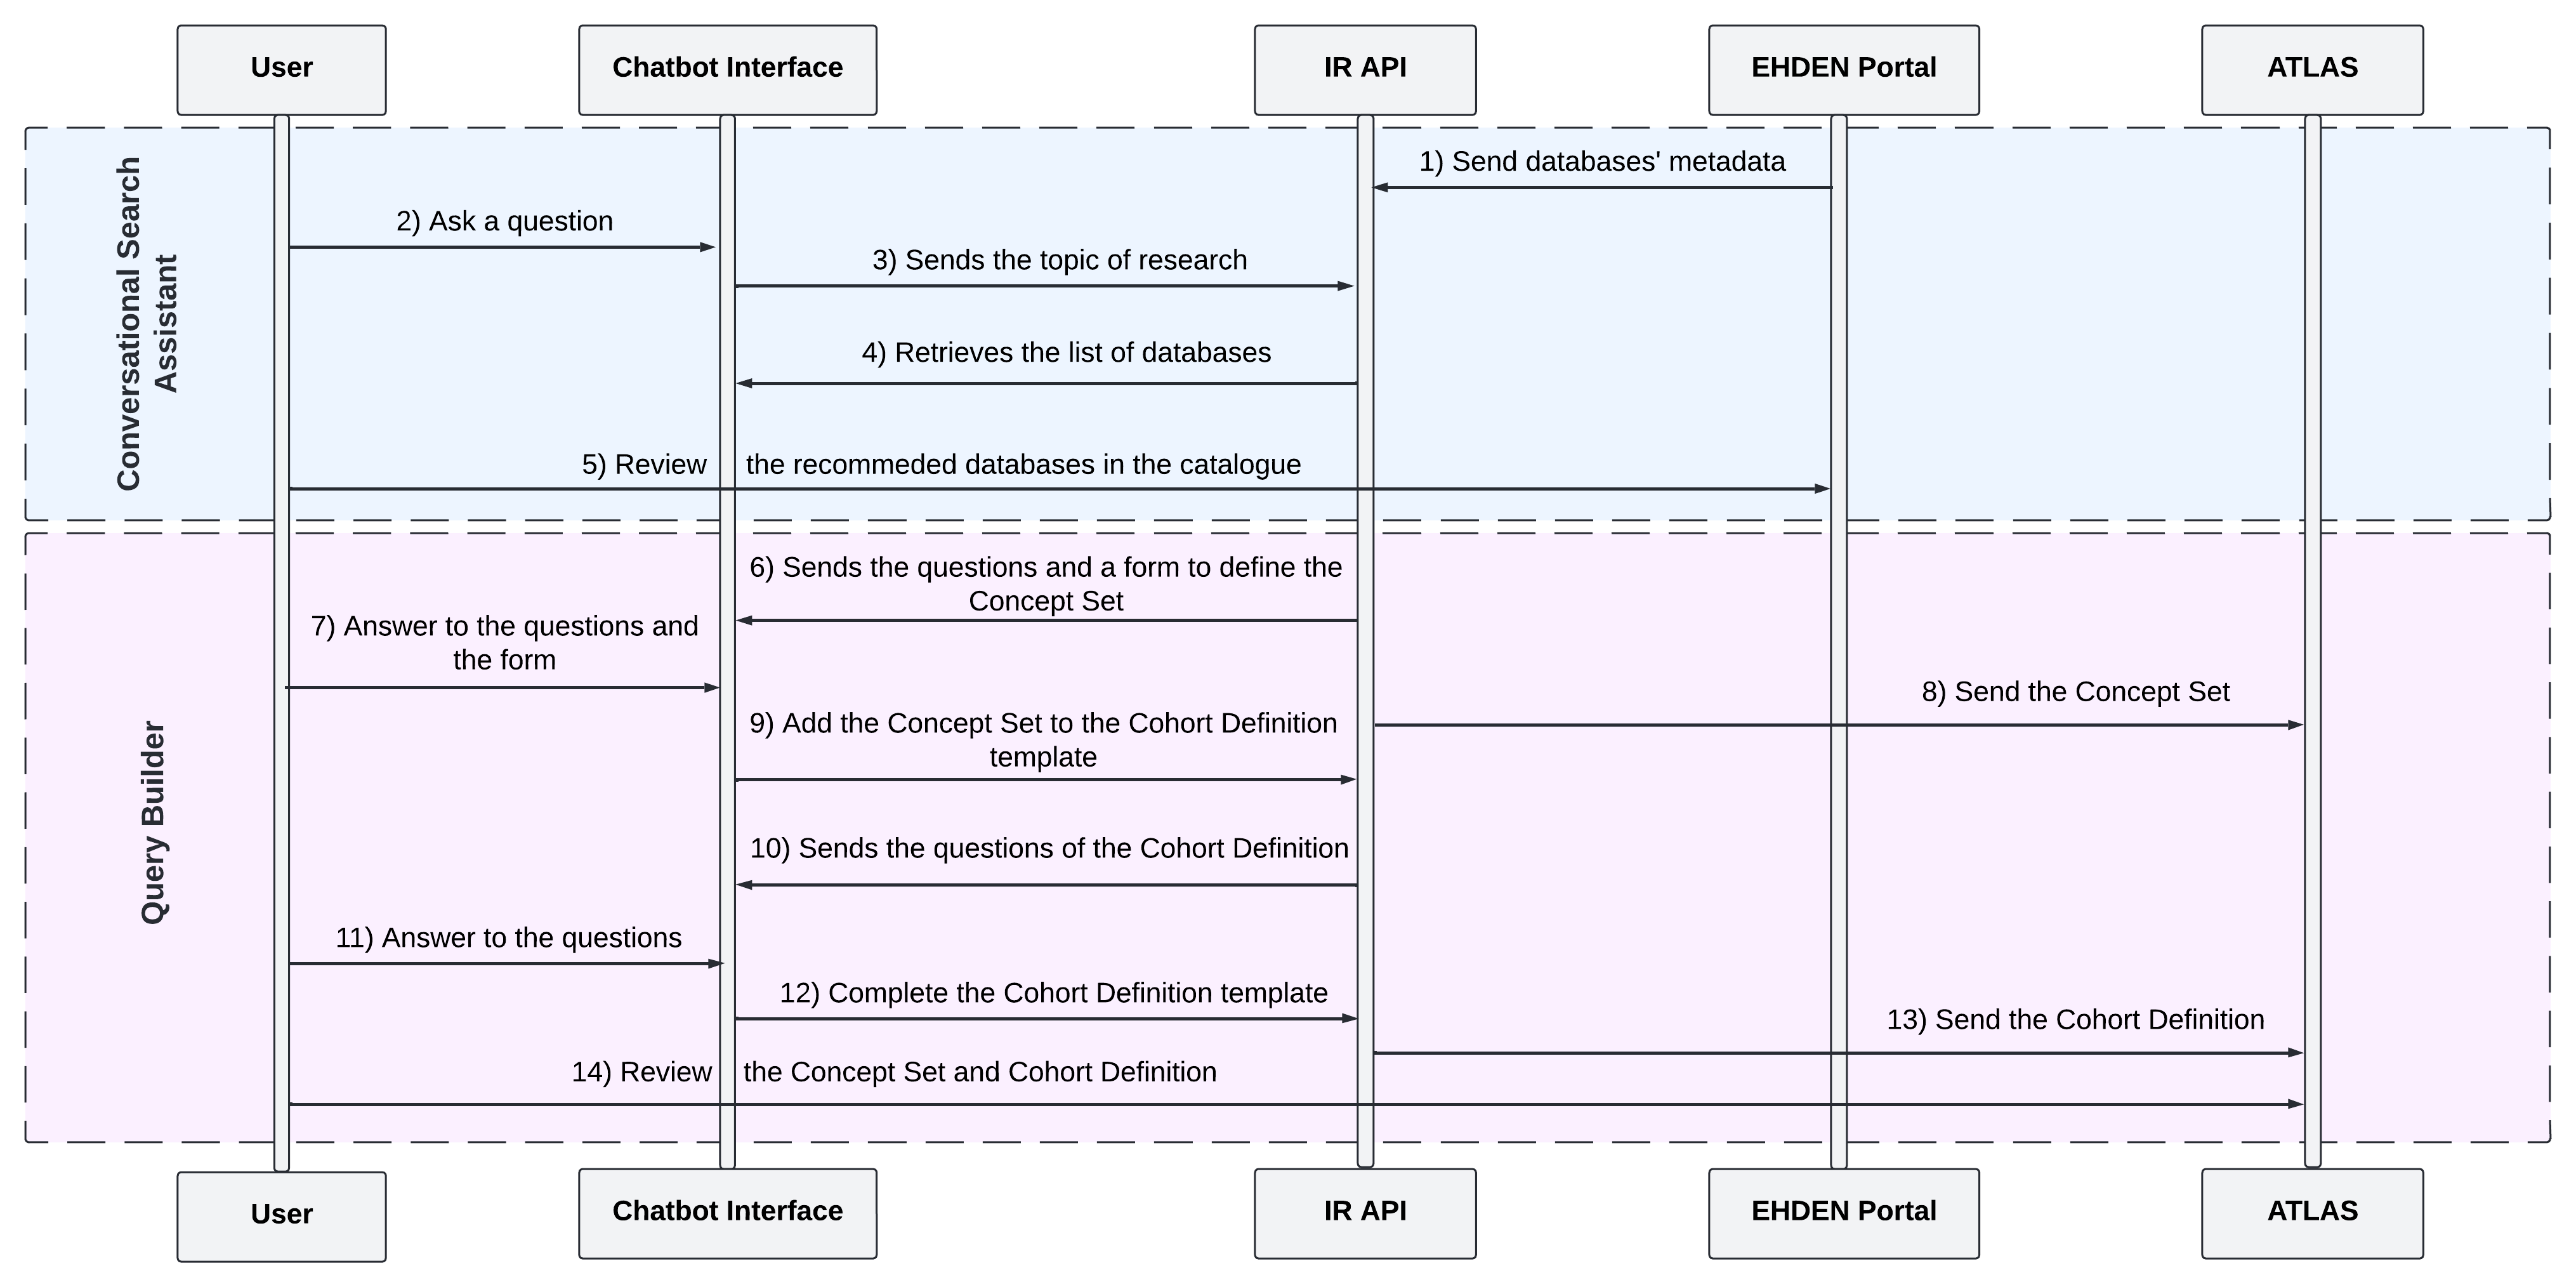
\includegraphics[width=\textwidth]{figs/chapter4/interaction_diagram.png}
  \centering
  \caption{Interaction diagram between the user, the system components and external tools.}
  \label{fig_interaction}
\end{figure}

This diagram presents all the interactions of the conversational query builder, not only presenting the interactions detailed in the previous chapter \ref{chapter:ConversationalSearchAssistant} — steps 1) to 5) —, but also the interactions that will be performed during the detail of this chapter — steps 6) to 9).

Reminding the interactions explained in chapter \ref{chapter:ConversationalSearchAssistant}, the {\ir} component receives the databases' metadata from the {\ehden} Portal — step 1) —, creating and indexing the documents. The user asks a question to the Chatbot Interface — step 2). Here, the {\llm} applies his task of identifying the research topic and sends it to the {\ir} API — step 3). The {\ir} API retrieves the most suitable databases for the research concept and sends the list of databases to the Chatbot Interface — step 4). The user can review the recommended databases in the catalogue in the {\ehden} Portal — step 5). 

Now, the query builder phase starts. The {\ir} API, when sending the databases to the chatbot interface, also sends a question to complete a field in the cohort definition — step 6). The user answer to the question — step 7) — and the {\llm}, in the Chatbot Interface, analyses if the user message is an answer to the question. If so, the answer will be saved in the cohort template — step 8). Steps 6), 7), and 8) are repeated until the cohort template is complete. Finally, the {\ir} API sends the cohort definition to ATLAS — step 9).



\subsection{Template and Questions}

The generated cohort definition, in the ATLAS platform, is in JSON format, which produces two crucial JSON files. One is the template for users to fill out during the conversation {\small\normalfont(\texttt{cohort\_template.json})}. This template is a copy of the cohort definition file without the cohort data {\small\normalfont(\texttt{cohort\_questions.json})}. The other file is the questions associated with each key field of the template. Each question should be simple and efficient so the medical researcher can respond to it, and its response is the value of that key. Also, each question in the template is manually inserted in the JSON file.  

% TODO: referenciar os templates


\begin{listing}[H]
  \begin{minted}[breaklines]{json}
      
  {
    "ConceptSets": [
      {
        "expression": {
            "items": "Do you have any other concepts to add to the concept set? (The question should be a yes with the new concepts or no response.)"
        }
      }
    ],
    "PrimaryCriteria": {
      "CriteriaList": [
        {
          "DrugExposure": {
            "CodesetId": 0,
            "First": true
          }
        }
      ],
      "ObservationWindow": {
        "PriorDays": "In terms of the observation window, what is the number of previous days? you can choose from 0, 1, 7, 14, 21, 30, 60, 90, 120, 180, 365, 548, 730 or 1095.",
        "PostDays": "In terms of the observation window, what is the number of days after? you can choose from 0, 1, 7, 14, 21, 30, 60, 90, 120, 180, 365, 548, 730 or 1095."
      },
      "PrimaryCriteriaLimit": {
        "Type": "First"
      }
    },
    "QualifiedLimit": {
      "Type": "First"
    },
    "ExpressionLimit": {
      "Type": "First"
    },

    (...)
  \end{minted}
  \caption{The cohort questions file {\small\normalfont(\texttt{cohort\_questions.json})}.}
  \label{questions}
  \end{listing}

\begin{listing}[H]
  \begin{minted}[breaklines]{json}
      
  {
    "ConceptSets": [
      {
        "expression": {
            "items": "Do you have any other concepts to add to the concept set? (The question should be a yes with the new concepts or no response.)"
        }
      }
    ],
    "PrimaryCriteria": {
      "CriteriaList": [
        {
          "DrugExposure": {
            "CodesetId": 0,
            "First": true
          }
        }
      ],
      "ObservationWindow": {
        "PriorDays": "In terms of the observation window, what is the number of previous days? you can choose from 0, 1, 7, 14, 21, 30, 60, 90, 120, 180, 365, 548, 730 or 1095.",
        "PostDays": "In terms of the observation window, what is the number of days after? you can choose from 0, 1, 7, 14, 21, 30, 60, 90, 120, 180, 365, 548, 730 or 1095."
      },
      "PrimaryCriteriaLimit": {
        "Type": "First"
      }
    },
    "QualifiedLimit": {
      "Type": "First"
    },
    "ExpressionLimit": {
      "Type": "First"
    },
    
    (...)
  \end{minted}
\caption{The cohort template file {\small\normalfont(\texttt{cohort\_template.json})}.}
\label{template}
\end{listing}  


\subsection{Template Pointer}

In a nutshell, the cohort questions file have the questions to complete the cohort template file. However, when exchanging messages with the user, tracking which questions must be asked and which question the user responded to is essential and also a problem.

The solution to this issue is creating a pointer to a template key. The pointer retrieves a template key that should be completed with the user information. The pointer points to the same key until the user responds to the question associated with the pointer. Otherwise, it moves to the following template key.

So, during the conversation, the pointer helps:

\begin{itemize}
  \item To determine the appropriate question to ask the user.
  \item To identify which key of the cohort template to use to save the user's answer.
  \item To move on to the next question of the cohort template.
\end{itemize}

This solution keeps track of the user's responses and dynamically updates the template with the relevant information throughout the conversation.


\section{Concepts Set}

% https://ohdsi.github.io/TheBookOfOhdsi/Cohorts.html#conceptSets

In template \ref{template}, a cohort is defined by multiple JSON fields. One of these fields is the concepts set (the template key is '\textit{ConceptsSet}'), which is a list of concepts required to meet the study requirements of the researcher. The definition of the concept set also needs to be defined in the conversation and so, the strategy was first define the concept set in the conversation and then, the remaining fields of the cohort template.

Before defining a cohort, the concept set needs to be determined. It is a set of standardized medical terms that define clinical elements such as diseases, drugs, and procedures.

This section details the creation of the concept set needed for the cohort definition later.


\subsection{Expression}
A concept set expression is comprised of a list of concepts with the following attributes:

\begin{itemize}
  \item \textbf{concept}: Definition of a concept, using data contained in the concepts file  {\small\normalfont(\texttt{concepts.csv})} (section \ref{data}).
  \item \textbf{isExcluded}: Exclude the concept from the concept set.
  \item \textbf{includeDescendants}: Add all of descendants of a concept, with it also included.
  \item \textbf{includeMapped}: Allow the search for non-standard concepts.
\end{itemize}


The JSON example \ref{conceptset} below represents a concept definition within a concept set expression. This example is not real information; it is just to define a concept set visually.

\begin{listing}[H]
  \begin{minted}[breaklines]{json}
      
    {
      "id": 0,
      "name": "costum_concept_set",
      "expression": {
          "items": [
              {
                  "concept": {
                      "CONCEPT_ID": 231256,
                      "CONCEPT_NAME": "Covid-19",
                      "DOMAIN_ID": "Condition",
                      "VOCABULARY_ID": "ASG67HR",
                      "CONCEPT_CLASS_ID": "ASG67 code",
                      "CONCEPT_CODE": "953635",
                      "VALID_START_DATE": "2000-01-01",
                      "VALID_END_DATE": "2099-12-31"
                  },
                  "isExcluded": false,
                  "includeDescendants": true,
                  "includeMapped": false
              },
              
              (...)
          ]
      }
    }

  \end{minted}
\caption{A Concept Set expression example.}
\label{conceptset}
\end{listing}  



\subsection{Implementation}


% 0) o utilizador insere uma query, o chatbot pergunta se ele tem mais conceitos, se sim, que os indique, até ao utilizador dizer que não tem mais conceitos para adicionar
% 1) utilizar IR para encontrar os conceitos associados à query que o user inseriu
% 2) ir buscar as informações adicionais aos ficheiro de conceitos
% 3) enviar a lista de conceitos ao utilizador e apresentar como forms 
% 4) utilizador escolhe os conceitos que quer inserir e escolhe os atributos
% 5) submete o forms, e a concept set é criado


The goal is to create a JSON object identical to the one in the example \ref{conceptset} with the concepts selected by the medical researcher.

When a user enters a query, the conversational search assistant retrieves the best databases related to the health topic of that query. It should also inquire whether the user has additional concepts for their study requirements. In an implementation vision, the first key to complete in the cohort template is '\textit{ConceptsSet}', so the question regarding that key is rewritten by the {\llm} and then asked to the user.

The user should respond to whether there are additional concepts to add. If there are, he should indicate them. If not, he should provide a negative answer. The chatbot will continue to ask if there are more concepts until the user confirms that there are no more to add.

Now, in the {\ir} component, the {\bm} technique searches in the collection for the concepts the user indicates in his responses. After identifying each concept in the collection using the {\ir} technique search, additional information from the concept file is added. This includes the concept ID, concept code, and other attributes that define the concept as represented in example \ref{conceptset}.

The list of concepts identified is sent to the chatbot interface. The chatbot interface shows the concepts in a form. For example, the Figure \ref{fig_forms} shows a form to create the concept set. The user selected which concepts he wants to include and the others attributes.

% TODO:  meter blur nos conceitos e ids
\begin{figure}[H]
  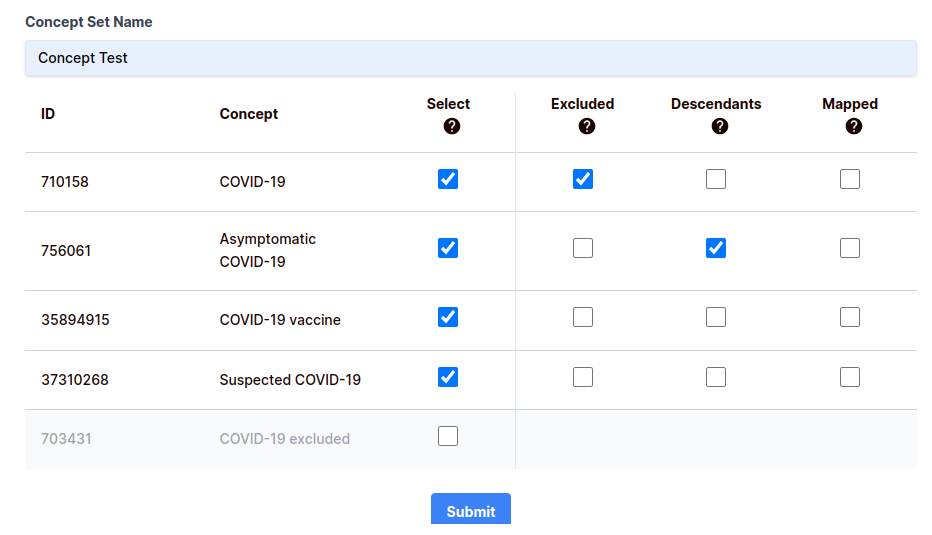
\includegraphics[width=1\textwidth]{figs/chapter4/form.png}
  \centering
  \caption{The form to create the Concept Set.}
  \label{fig_forms}
\end{figure}

Finally, the user submits the forms, creating the concept set. The chatbot sends a message informing the user that he can download the cohort, which is now only the concept set. The pointer of the cohort template moves to the next key.



\section{Cohort Definition}

% depois do concept set estar definido, o template pointer passa para a proxima key com pergunta
% o LLM gera a pergunta e a interface apresenta-a ao utilizador
% o utilizador responde 
% o LLM verifica se a mensagem do utilizador é em resposta à pergunta
%   - se sim, atualiza o template com a resposta, e o template pointer avança
%   - se não, volta a questionar a mesma questão ao utilzador
% este ciclo repete-se até o cohort estar completo


% TODO: intro, e fazer refenciar o template

Once the concept set is defined, the list of concepts and their attributes are saved on the template, where the template key points to. Then, the template pointer moves to the next template key. The {\llm} generates a specific question related to the question that the current key points to. This generated question is then presented to the user through the interface.

The user provides a response to the question presented. The user message could be a possible response to the question or, for example, can be a random message. So, the {\llm} checks if the user's message is indeed an answer to the question. This task is mentioned in the section \ref{sec:llm}. If the response is valid,the {\llm} extracts the value and the template is updated with that value. The template pointer advances to the next key, where the next question will be generated by the {\llm}. Otherwise, if the response is invalid or unrelated, the pointer remains on the same key because the question is not answered yet.

This cycle of getting the question of the pointer, generating the question, presenting it, receiving a response, and verifying the response repeats until the entire cohort is complete, and all keys in the template are filled with the appropriate user responses.

% TODO: end



\section{ATLAS ...}


% tbd
nome da secção

o que escrever aqui

onde meter esta figura

\begin{figure}[H]
  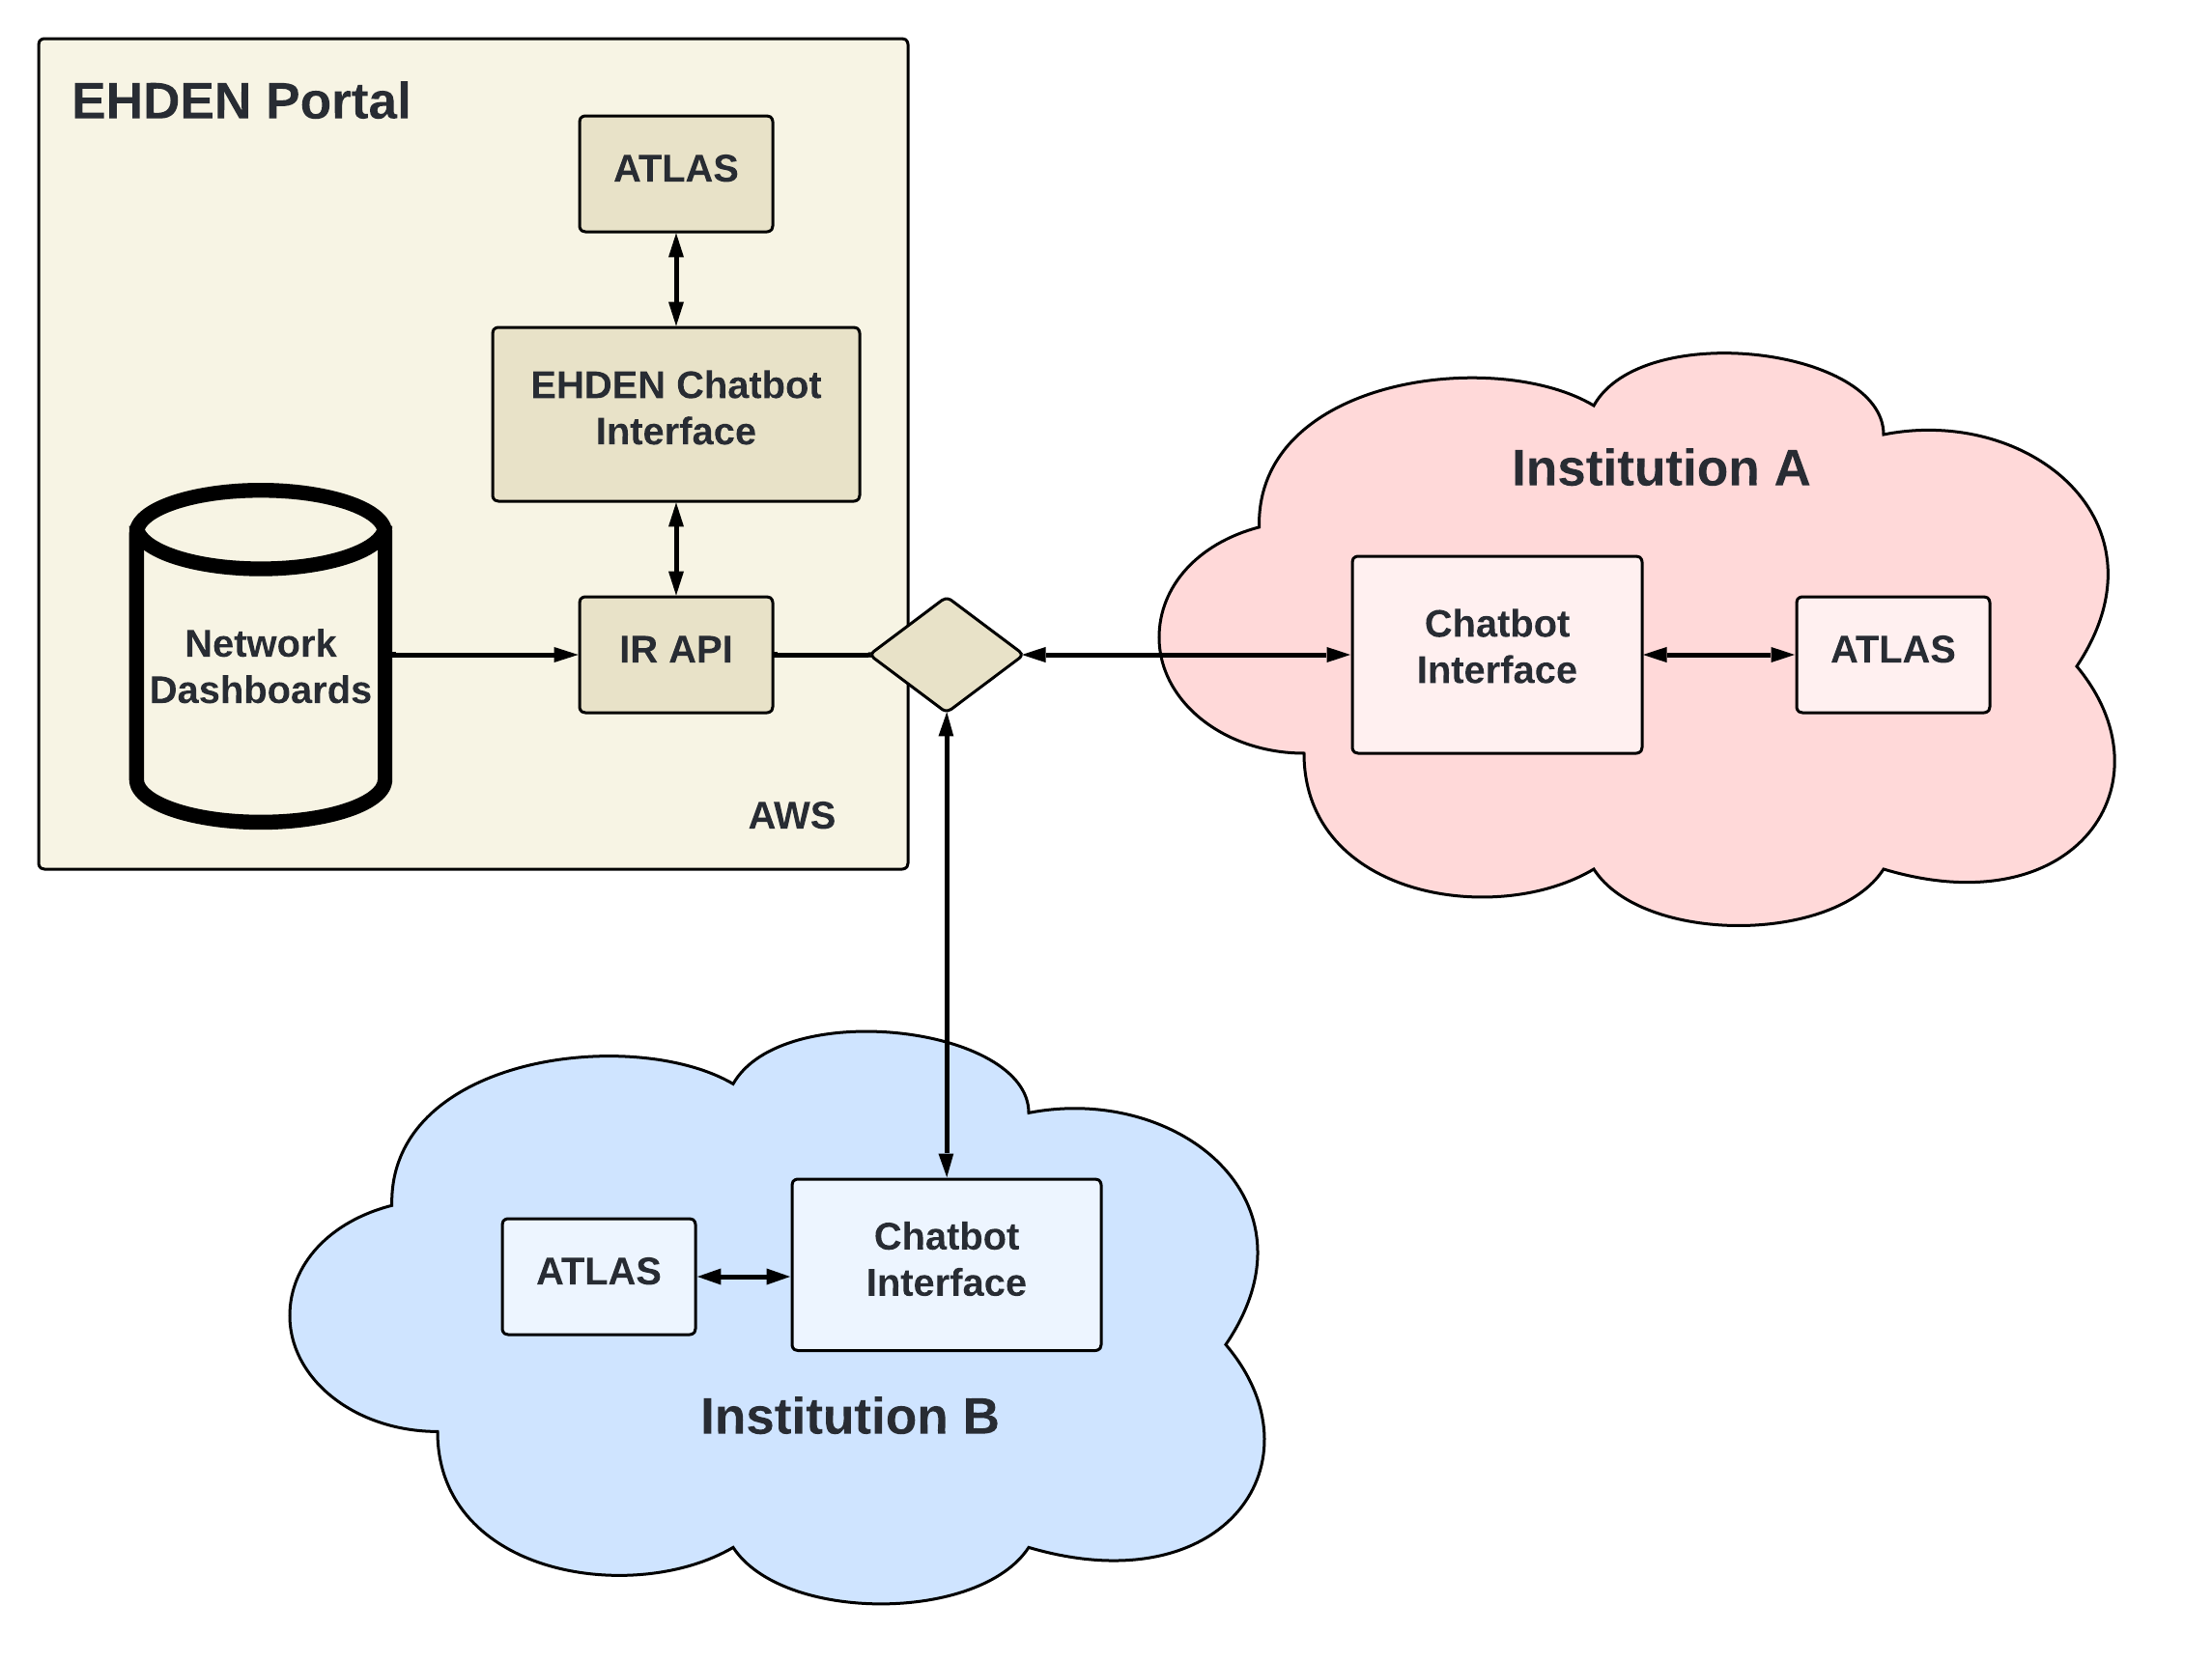
\includegraphics[width=0.5\textwidth]{figs/chapter4/network_diagram.png}
  \centering
  \caption{Network diagram.}
  \label{fig_network}
\end{figure}


---

o que fazer com os json dos templates

quero refenciar o artigo cbms e o MIE


----

falta falar que há um histórico para guardar as conversas de investigadores médico --> onde meto isto?

é preciso meter uma documentação da API?

%%%%%%%%%%%%%%%%%%%%%%%%%%%%%%%%%%%%%%%%%%%%%%%%%%%%%%%
% End of Thesis text 
%%%%%%%%%%%%%%%%%%%%%%%%%%%%%%%%%%%%%%%%%%%%%%%%%%%%%%%

\backmatter

%%%%%%%%%%%%%%%%%%%%%%%%%%%%%%%%%%%%%%%%%%%%%%%%%%%%%%%
% Print all used references
%%%%%%%%%%%%%%%%%%%%%%%%%%%%%%%%%%%%%%%%%%%%%%%%%%%%%%%

\begingroup
\renewcommand{\bibfont}{\footnotesize}
% Redefine References name to Portuguese
% Change if you are using english
\defbibheading{bibliography}[References]{
	\chapter{#1}
}
\SingleSpacing
\setlength\bibitemsep{8pt}
\printbibliography[heading=bibliography]
\endgroup


%%%%%%%%%%%%%%%%%%%%%%%%%%%%%%%%%%%%%%%%%%%%%%%%%%%%%%%
% Load appendix
%%%%%%%%%%%%%%%%%%%%%%%%%%%%%%%%%%%%%%%%%%%%%%%%%%%%%%%

\mainmatterWithoutReset
\appendix

\include{chapters/appendix-more}

\end{document}
